%        File: ans_2013_therm_pres.tex
%     Created: Thu Jun 13 02:00 PM 2013 C
% Last Change: Thu Jun 13 02:00 PM 2013 C
%
%\documentclass[11pt,handout]{beamer}

\documentclass[9pt]{beamer}
\usetheme[white]{Wisconsin}
%\title[short title]{long title}
\title[Thermal Analysis in Cyder]{Dynamic Determination of Thermal Repository Capacity for Fuel Cycle Analysis} 
%\subtitle[short subtitle]{long subtitle}
\subtitle[ANS 2013]{American Nuclear Society Annual Conference 2013}
%\author[short name]{long name}
\author[K. Huff]{Kathryn Huff$^1$ \& Alexander Bara$^2$}
%\date[short date]{long date}
\date[6.18.2013]{June 18, 2013}
%\institution[short name]{long name}
\institute[UW-Madison\&ANL]{$^1$U. Wisconsin-Madison \& $^{1,2}$Argonne National 
Laboratory}

\usepackage{amsfonts}
\usepackage{amsmath}
\usepackage{xspace}
\usepackage{graphicx}
\usepackage{subfigure}
\usepackage{booktabs} % nice rules for tables
\usepackage{microtype} % if using PDF
\usepackage{bigints}
\newcommand{\units}[1] {\:\text{#1}}%
\newcommand{\SN}{S$_N$}%{S$_\text{N}$}%{$S_N$}%
\DeclareMathOperator{\erf}{erf}
\newcommand{\Cyder}{\textsc{Cyder}\xspace}
%I need some complimentary error funcitons\ldots 
\DeclareMathOperator{\erfc}{erfc}
%page numbers
\setbeamertemplate{footline}[page number]
\setbeamertemplate{caption}[numbered]
%Those icons in the references are terrible looking
\setbeamertemplate{bibliography item}[text]

\begin{document}
%%%%%%%%%%%%%%%%%%%%%%%%%%%%%%%%%%%%%%%%%%%%%%%%%%%%%%%%%%%%%
%% From uw-beamer Here's a handy bit of code to place at 
%% the beginning of your presentation (after \begin{document}):
\newcommand*{\alphabet}{ABCDEFGHIJKLMNOPQRSTUVWXYZabcdefghijklmnopqrstuvwxyz}
\newlength{\highlightheight}
\newlength{\highlightdepth}
\newlength{\highlightmargin}
\setlength{\highlightmargin}{2pt}
\settoheight{\highlightheight}{\alphabet}
\settodepth{\highlightdepth}{\alphabet}
\addtolength{\highlightheight}{\highlightmargin}
\addtolength{\highlightdepth}{\highlightmargin}
\addtolength{\highlightheight}{\highlightdepth}
\newcommand*{\Highlight}{\rlap{\textcolor{HighlightBackground}{\rule[-\highlightdepth]{\linewidth}{\highlightheight}}}}
%%%%%%%%%%%%%%%%%%%%%%%%%%%%%%%%%%%%%%%%%%%%%%%%%%%%%%%%%%%%%
%%--------------------------------%%
\frame{
  \titlepage
}
%%--------------------------------%%
\AtBeginSection{
\begin{frame}
\frametitle{Outline}
\tableofcontents[currentsection]
\end{frame}
}

\section{Motivation}

\subsection{Current Fuel Cycle Simulator Tools}

% They just report mass flows
% or are proprietary and super long running

\begin{frame}[ctb!]
  \frametitle{Top Level Fuel Cycle Simulators}
  % most only report mass flows.
  \begin{figure}[htbp!]
    \begin{center}
      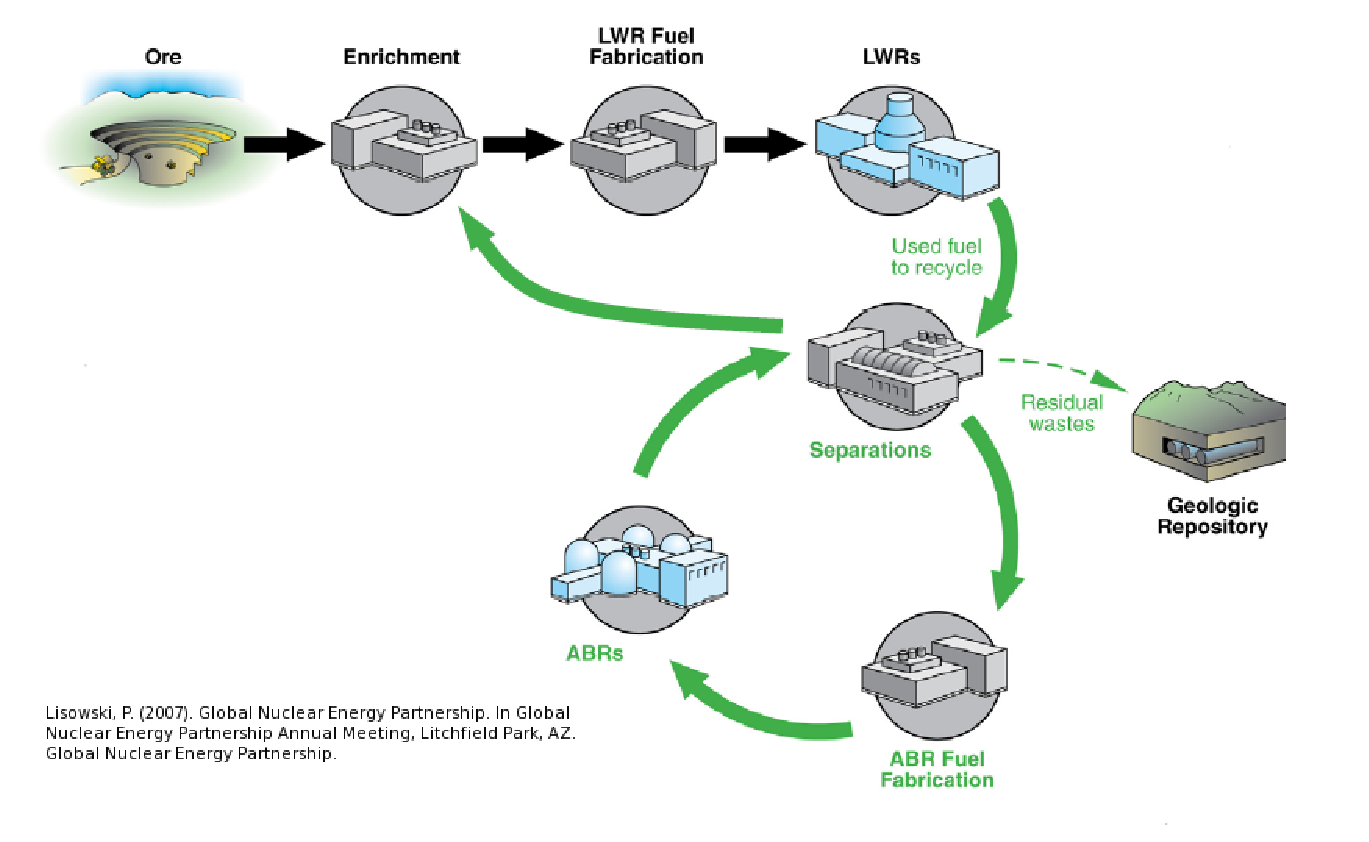
\includegraphics[height=4cm]{./images/simulations.eps}
    \end{center}
    \caption{Top level simulators are intended to model the collective 
    behavior of various fuel cycle decisions and 
    strategies \cite{lisowski_global_2007}.}
    \label{fig:simulation}
  \end{figure}
\end{frame}

\begin{frame}[ctb!]
  \frametitle{Need For an Integrated Repository Model}
  \footnotesize{
  % Incorporates disposal system decisions into metrics information
  % Captures Feedbacks
  Most current fuel cycle simulators neglect disposal system decisions and 
  repository behavior. 
  %        File: systools_tab.tex
%     Created: Mon Aug 29 09:00 AM 2011 C
% Last Change: Mon Aug 29 09:00 AM 2011 C
%
\begin{table}
  \centering
  \footnotesize{
  \begin{tabular}{|l|l|c|c|c|}
    \multicolumn{5}{c}{\textbf{Repository Capabilities within Systems Analysis Tools}}\\
    \hline
    Tool & Institution & Fuel Disposition & Radionuclide Transport & Heat Transport  \\
    \hline
    NUWASTE\cite{abkowitz_nuclear_2010} & NWTRB & yes & no & no \\
    VISION \cite{yacout_vision_2006} & INL   & yes & no & YMR only \\
    DANESS \cite{van_den_durpel_daness:_2006} & ANL   & no & no & no \\
    COSI   \cite{boucher_international_2010} & CEA   & yes & no & yes \\
    NFCSim \cite{schneider_nfcsim_2004} & LANL  & no & no & no \\
    CAFCA  \cite{guerin_benchmark_2009} & MIT   & no & no & no \\
    ORION  \cite{guerin_benchmark_2009} & BNL   & no & no & no \\
    \hline
  \end{tabular}
  \caption[System Tools]{System tools are lacking in radionuclide transport and  
  heat transport calculations in generic geolgies.}
  \label{tab:systools}
  }
\end{table}



}

\end{frame}


\subsection{Fuel Cycle Options}

\begin{frame}[ctb!]
  \frametitle{Future Fuel Cycle Options}
       % Future Fuel Cycles
    \begin{table}
      \centering
      \footnotesize{
      \begin{tabular}{|l|l|l|}
        \multicolumn{3}{c}{\textbf{Domestic Fuel Cycle Options}}\\
        \hline
        Title & Description& Challenges \\
        \hline
        \hline
        Open          & Once Through         & High Temperatures, Volumes \\
                      & Current US PWR Fleet &      \\
                      & No Separations       &      \\
                      & No Recycling         &      \\
                      & Higher Burnups &      \\
        \hline
        Modified Open & Partial Recycling     & Both high volumes \\
                      & Next Gen. PWR Fleet   &   and variable spent fuel streams \\
                      & Limited Separations   &      \\
                      & Limited Transmutation &      \\
                      & Advanced Fuel Forms   &      \\
                      & HLW treatment         &      \\
        \hline
        Closed        & Full Recycling       & Variable spent fuel streams \\
                      & Full Separations &      \\
                      & Full Recycling &      \\
                      & VHTGR, SFRs, &      \\
                      & other transmutation & \\
                      & HLW treatment  &      \\
        \hline
      \end{tabular}
      \caption[Fuel Cycle Options]{Domestic Fuel Cycle Options }
      \label{tab:fco}
      }
    \end{table}

\end{frame}

\subsection{Repository Concepts}



\begin{frame}[ctb!]
  \frametitle{Disposal Geology Options Considered}
   \begin{minipage}{0.44\textwidth}
     \begin{figure}[h!]
         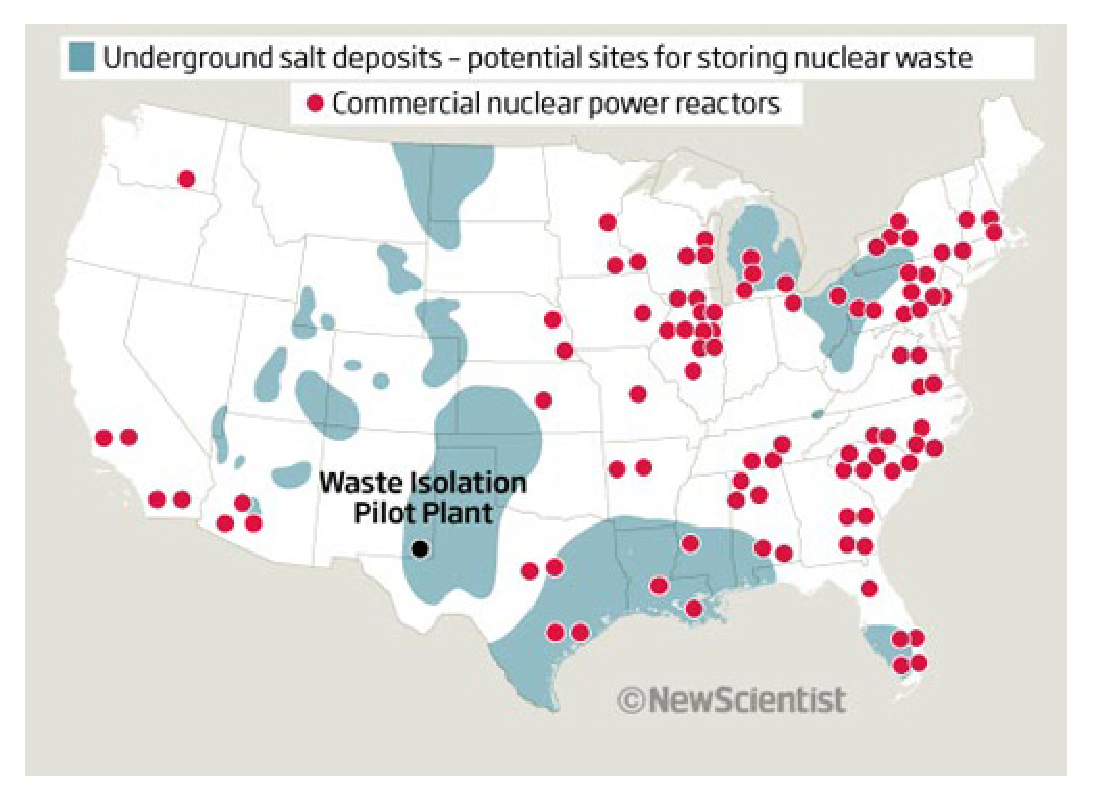
\includegraphics[width=0.8\textwidth]{./images/saltNewScientist.eps}
         \caption{U.S. Salt Deposits, ref. \cite{newscientist_where_2011}.}
     \end{figure}
     \begin{figure}[h!]
         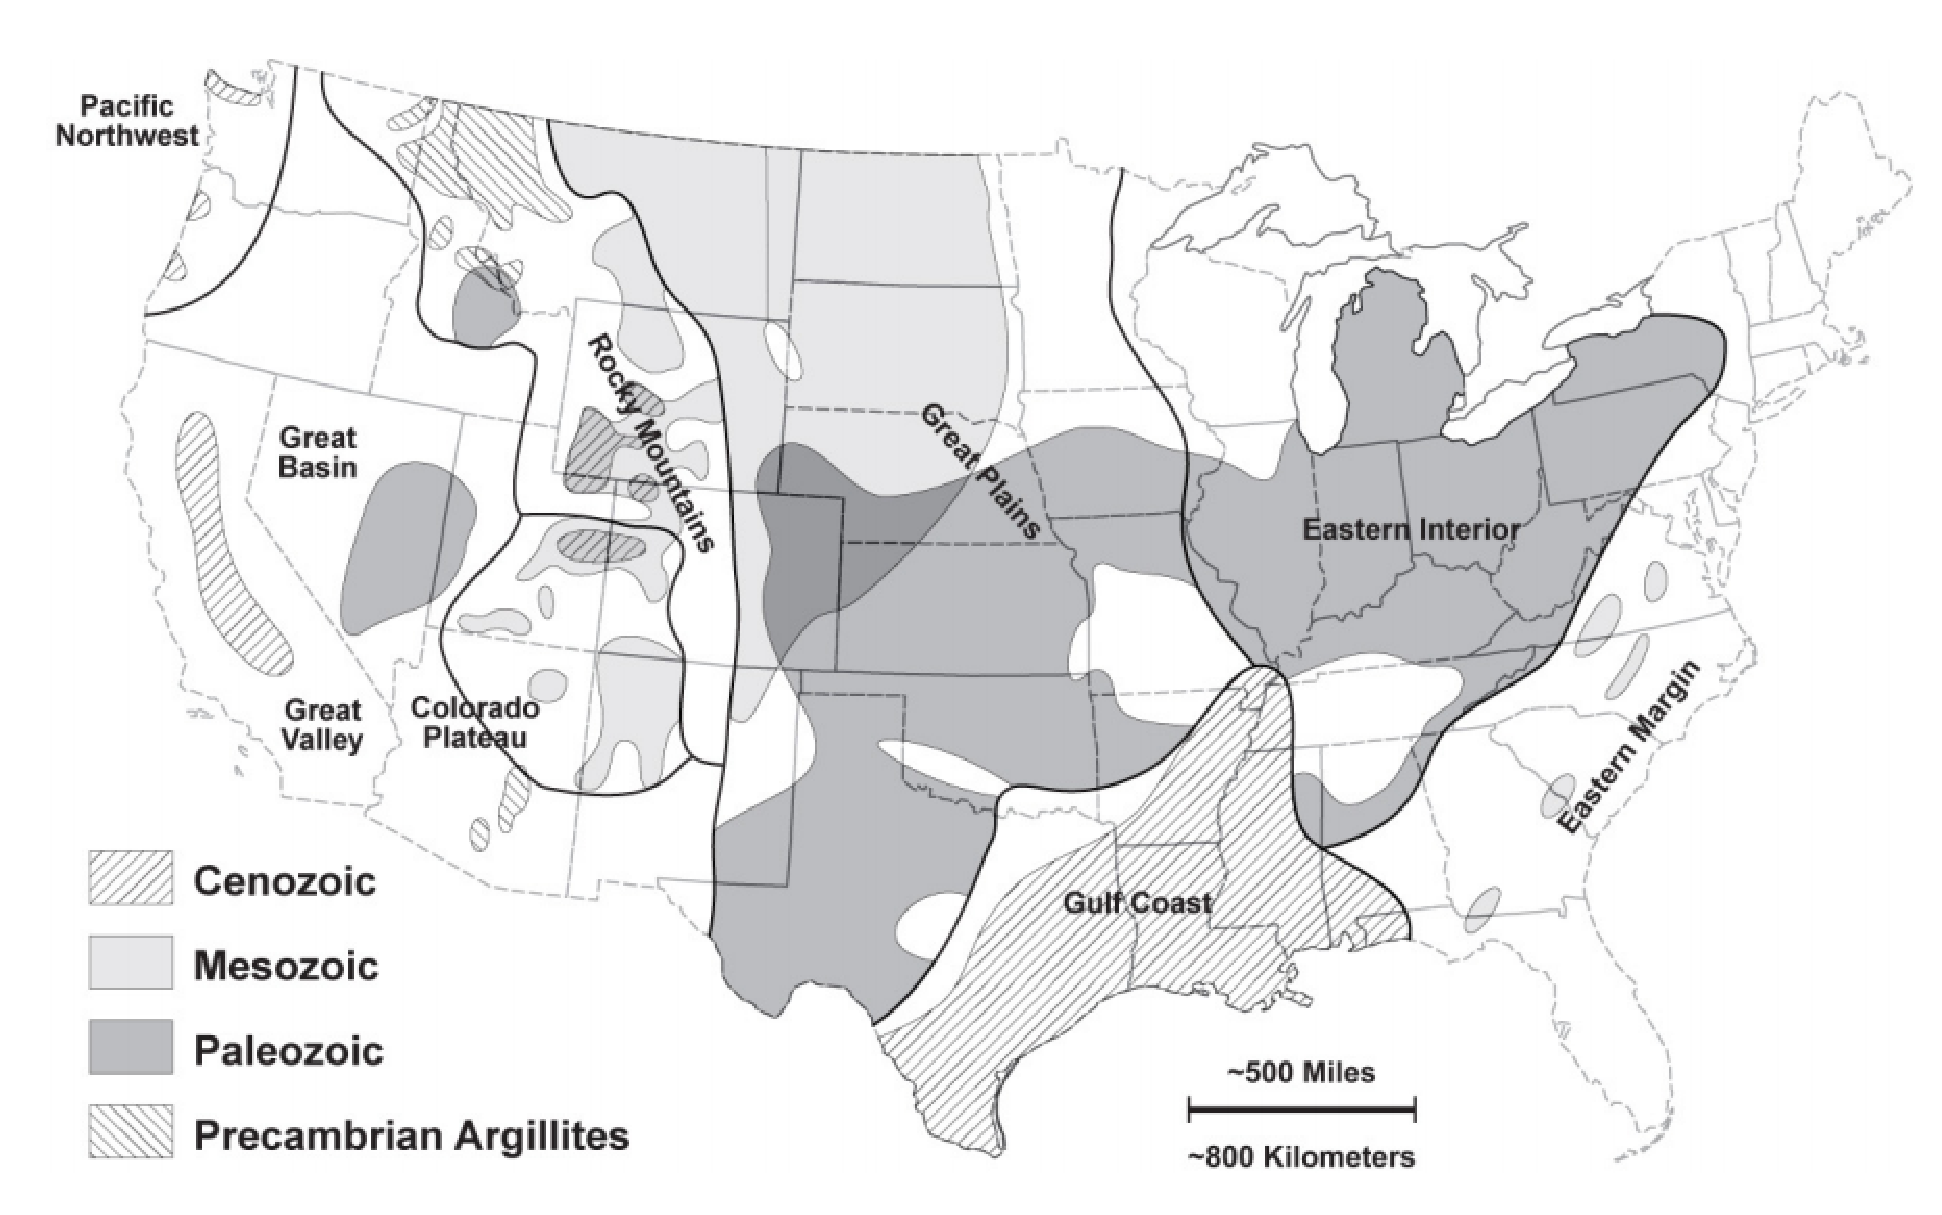
\includegraphics[width=0.8\textwidth]{./images/clayGonzales.eps}
         \caption{U.S. Clay Deposits, ref. \cite{gonzales_shales_1985}.}
     \end{figure}
   \end{minipage}
   \begin{minipage}{0.44\textwidth}
     \begin{figure}[h!]
         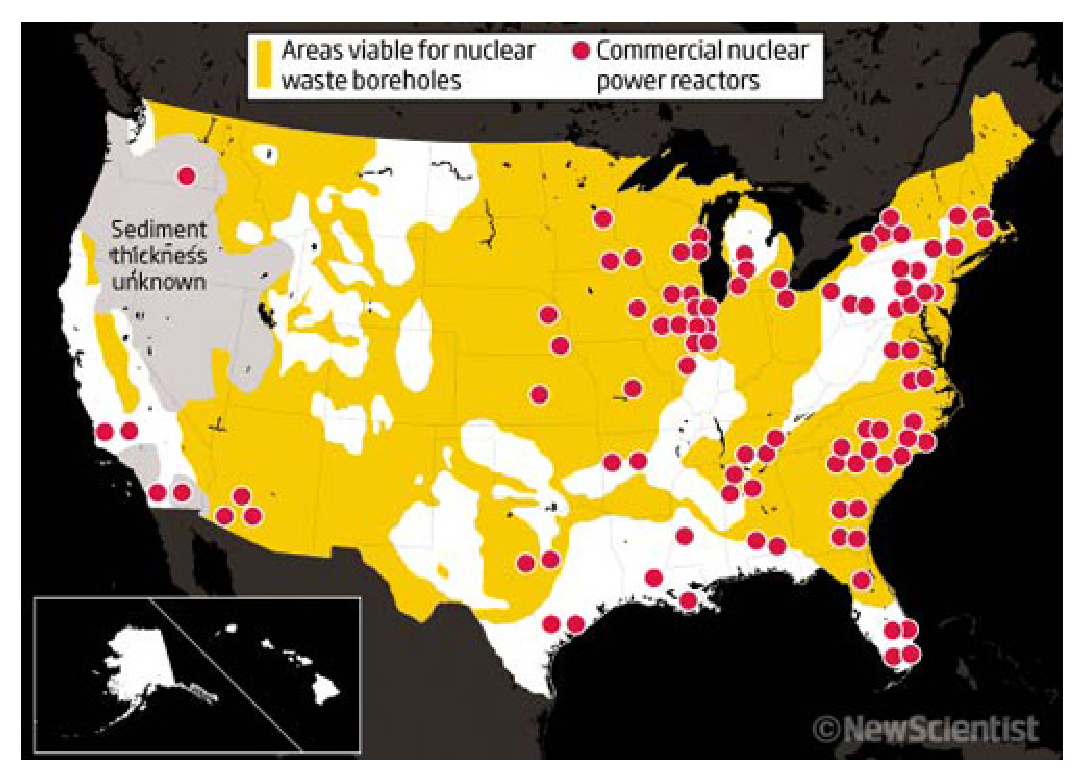
\includegraphics[width=0.8\textwidth]{./images/boreholeNewScientist.eps}
         \caption{U.S. Crystalline Basement, ref.  \cite{newscientist_where_2011}.}
     \end{figure}
     \begin{figure}[h!]
         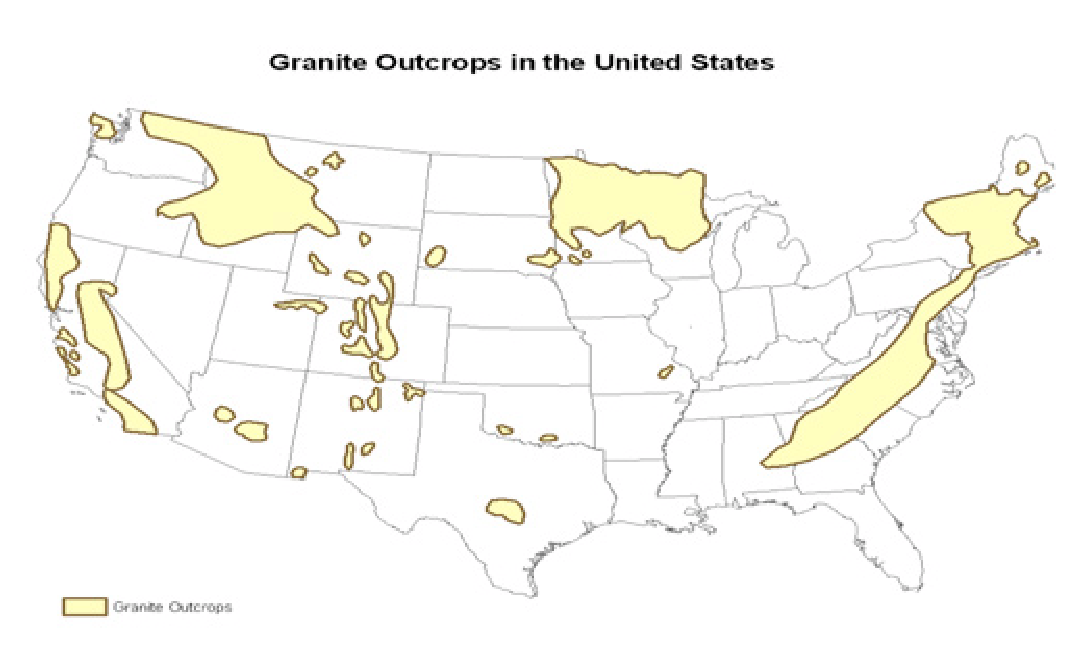
\includegraphics[width=0.8\textwidth]{./images/graniteBush.eps}
         \caption{U.S. Granite Beds, ref. \cite{bush_economic_1976}.}
     \end{figure}
   \end{minipage}
\end{frame}



%%----------------------------------------%%
\begin{frame}[ctb!]
  \frametitle{Repository Components}
\footnotesize{
  \begin{figure}[htbp!]
  \begin{center}
    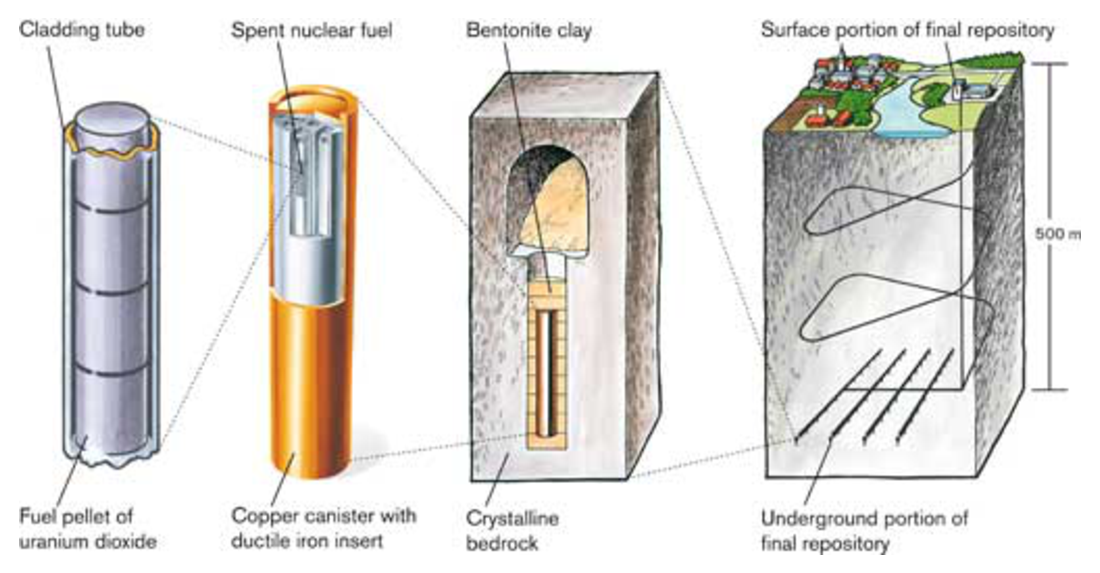
\includegraphics[width=0.7\textwidth]{./images/skb_components.eps}
  \end{center}
  \caption{Geologic disposal systems typically employ engineered barrier 
    systems as well as natural barrier systems. This is a Swedish concept in 
    granite \cite{ab_long-term_2006}.}
  \label{fig:skb_components}
\end{figure}

}
\end{frame}

\begin{frame}
  \frametitle{Repository Layouts}

  \begin{minipage}{0.49\textwidth}
    \begin{figure}[h!]
      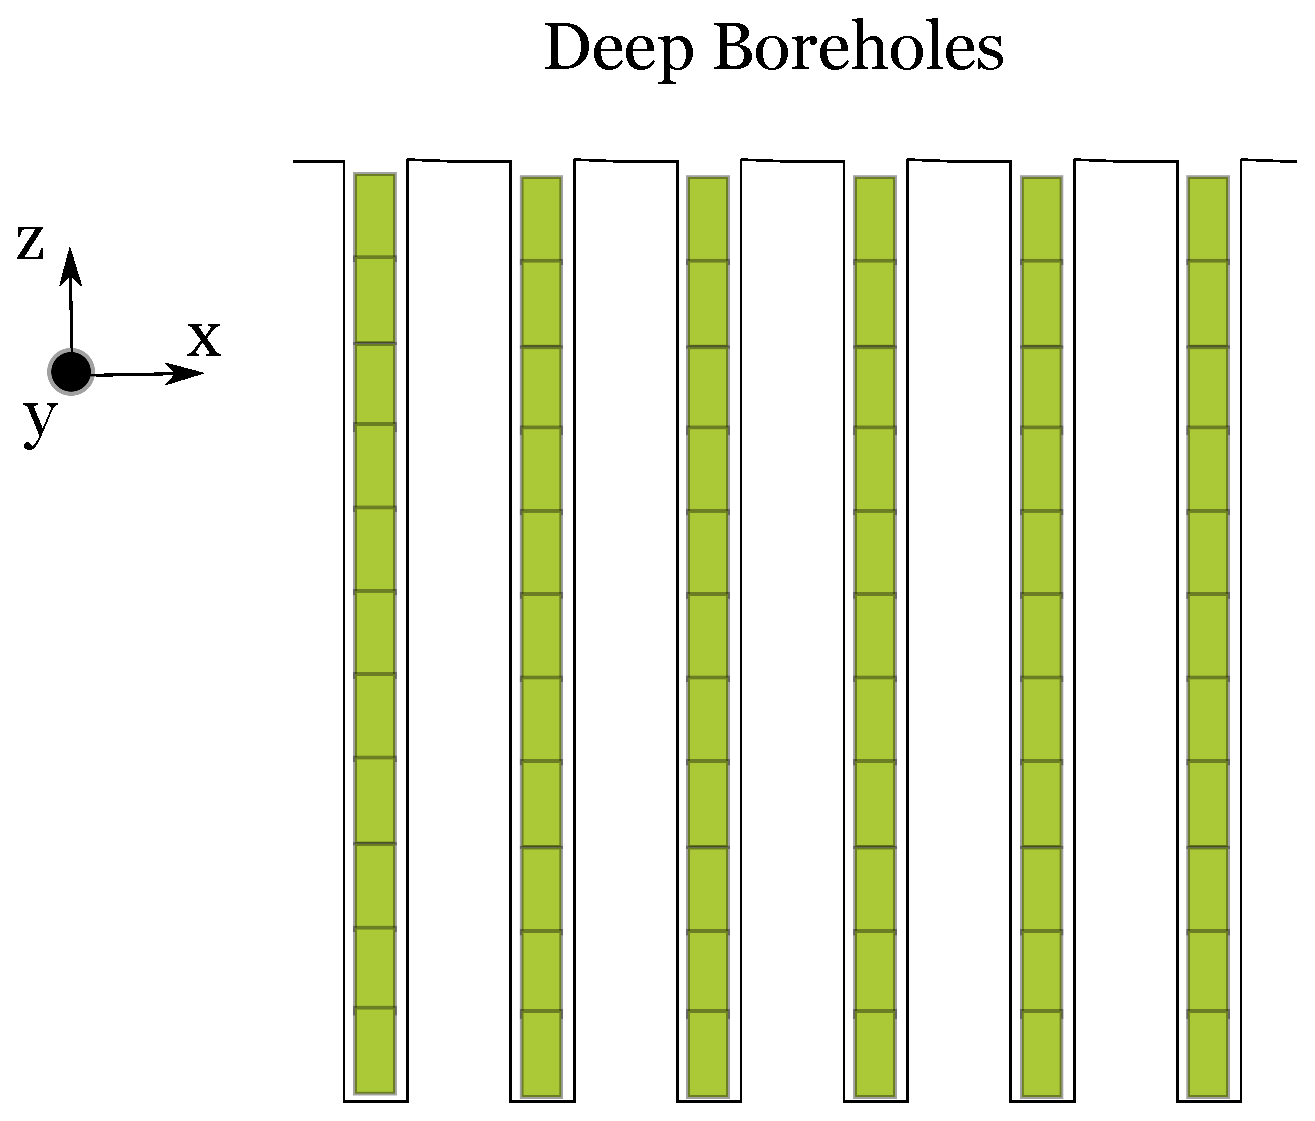
\includegraphics[width=0.75\textwidth]{./images/boreholes.eps}
    \end{figure}
    \begin{figure}[h!]
      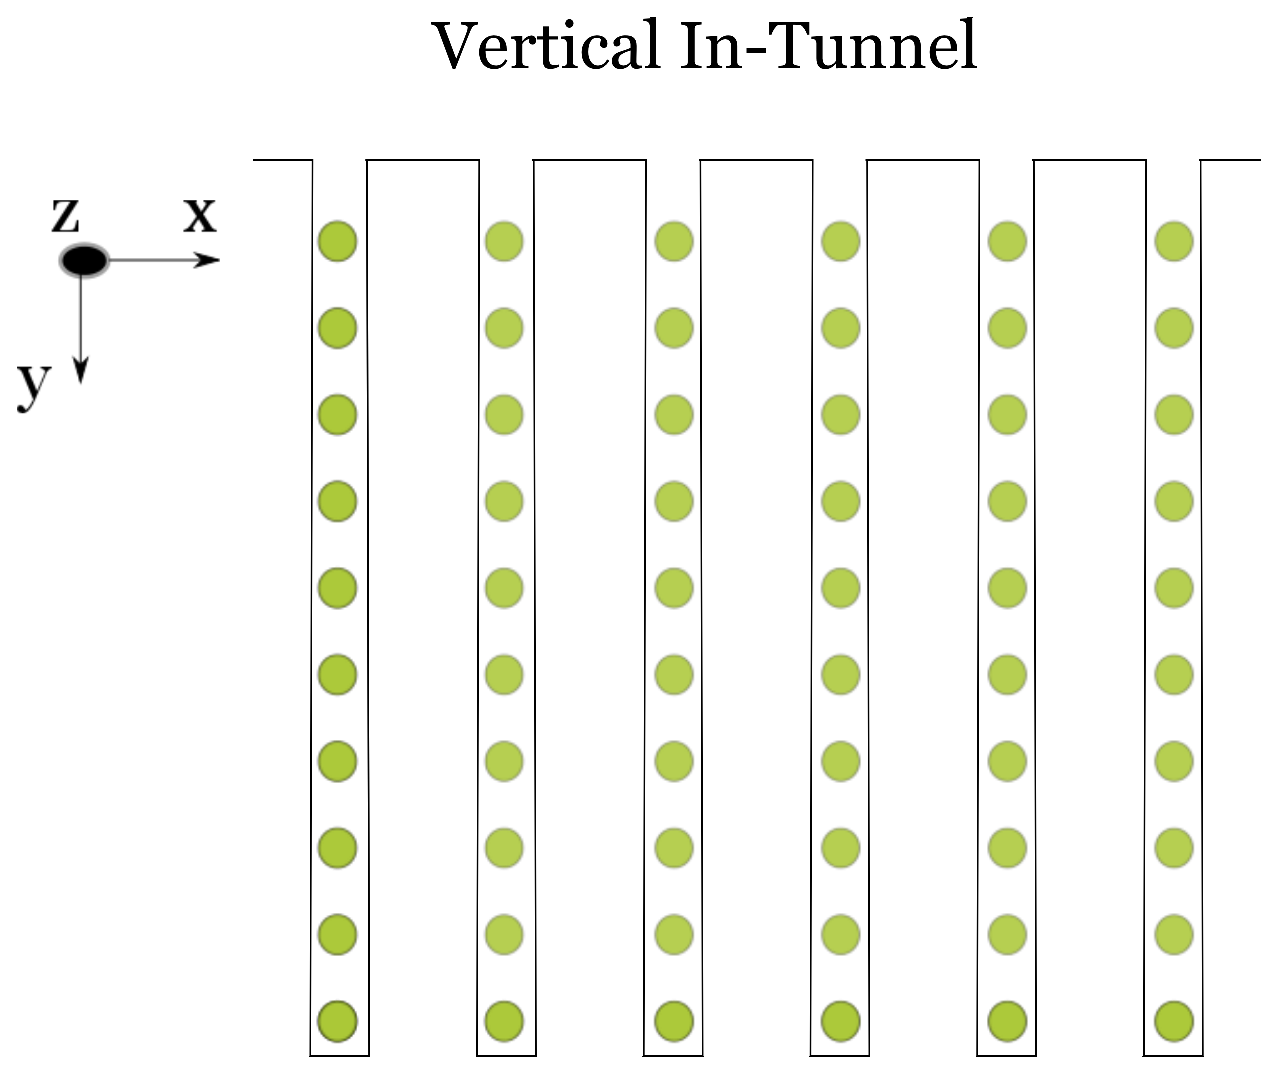
\includegraphics[width=0.75\textwidth]{./images/vertical.eps}
    \end{figure}
  \end{minipage}
  \hspace{0.01cm}
  \begin{minipage}{0.49\textwidth}
    \begin{figure}[h!]
      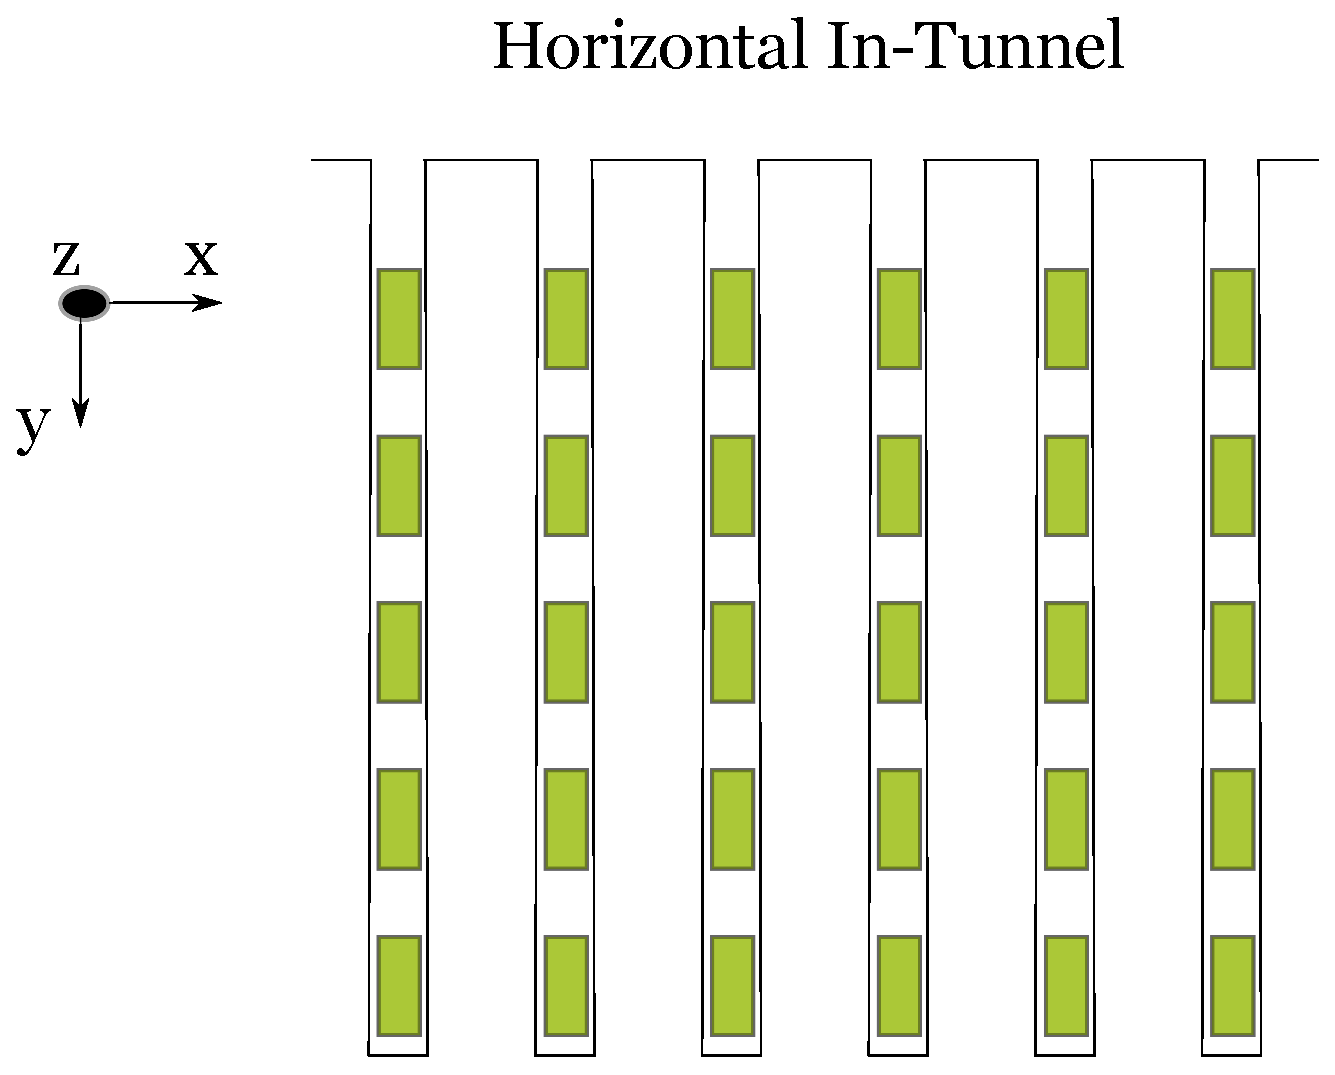
\includegraphics[width=0.8\textwidth]{./images/horizontal.eps}
    \end{figure}
    \begin{figure}[h!]
      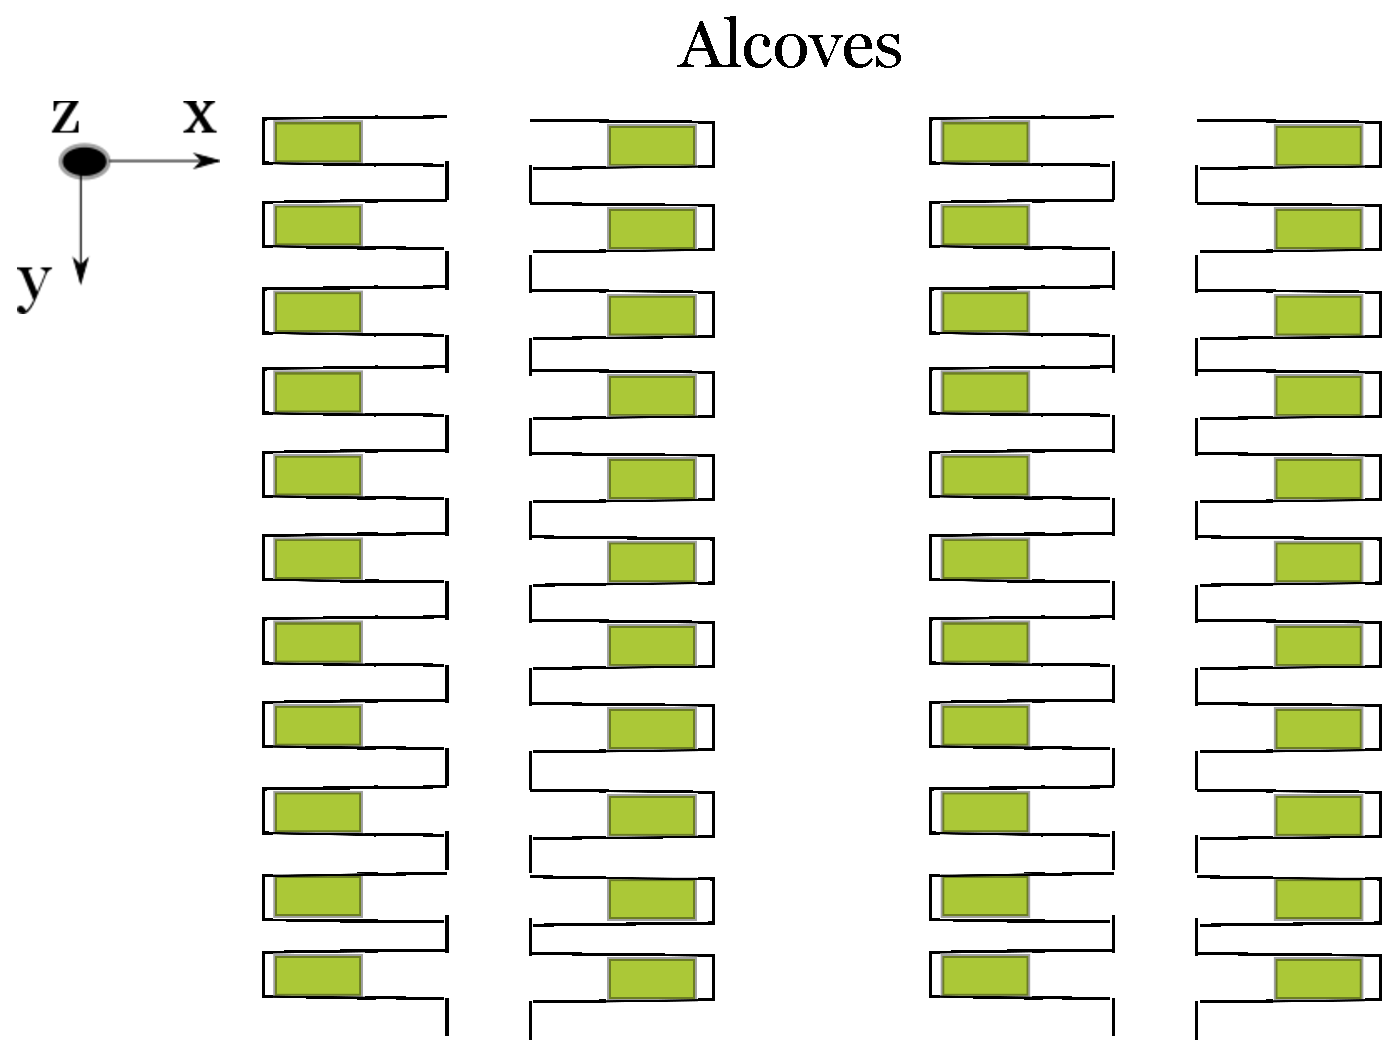
\includegraphics[width=0.8\textwidth]{./images/alcoves.eps}
    \end{figure}
  \end{minipage}

\end{frame}


\section{Modeling Paradigm}
\subsection{Cyder Modeling Paradigm}

\begin{frame}[ctb!]
  \frametitle{Cyder Paradigm : Modularity }
  A modular repository framework facilitates 
  \begin{itemize}
    \item  interchangable subcomponents (e.g. buffer material) so that 
      the impact on the disposal system performance may be observed
    \item and simulations with varying levels of detail.
  \end{itemize}
 \pause
  Integration with a fuel cycle simulator facilitates
  \begin{itemize}
    \item analysis of feedback effects upon the fuel cycle
    \item and investigation of fuel cycle choices on disposal system 
      performance.
  \end{itemize}
\end{frame}


\begin{frame}[ctb!]
  \frametitle{Cyder Paradigm : Waste Stream Acceptance}
  \footnotesize{
  
To participate in fuel cycle simulation, the repository model must accept arbitrary 
spent fuel and high level waste streams. 
  \begin{figure}[htbp!]
    \begin{center}
      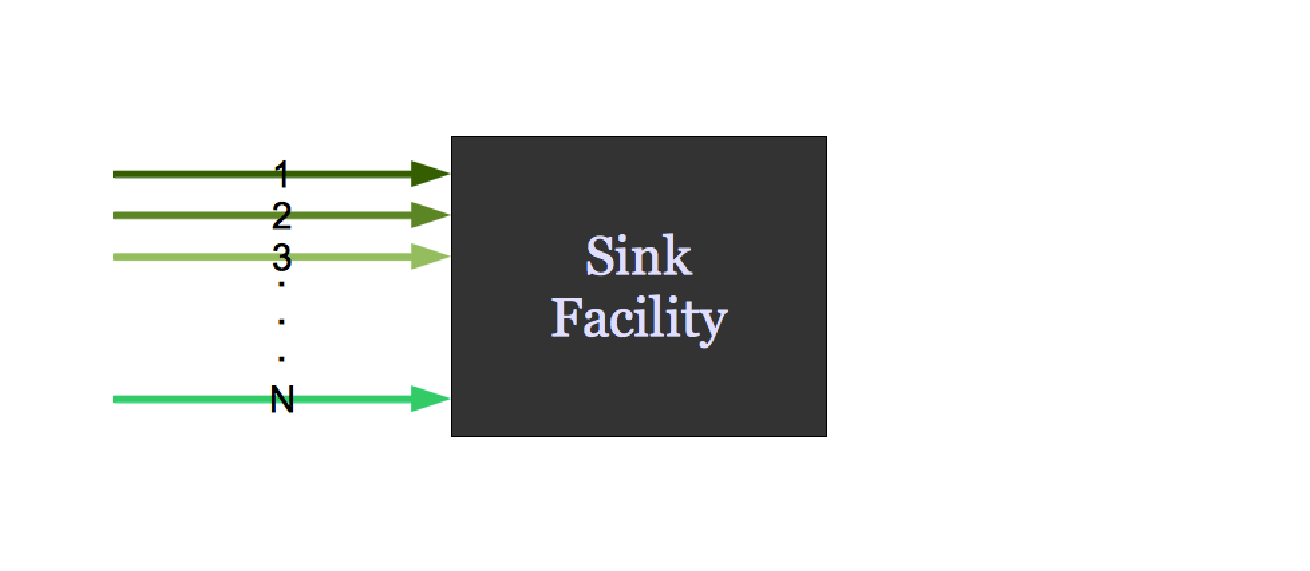
\includegraphics[height=5cm]{./images/sinkfacility.eps}
    \end{center}
    \caption{ The Cyder Facility dynamically accepts material from the coupled 
    fuel cycle simulation.  A waste stream is a material data object resulting 
    from the Cyclus simulated fuel cycle.  } 
    \label{fig:sinkfacility}
  \end{figure}
% Sink Facility ?
}
\end{frame}

\subsection{Thermal Modeling Paradigm}
\begin{frame}[ctb!]
\frametitle{Thermal Modeling in Cyder}
Two types of thermal modeling occur in Cyder. 
\begin{itemize}
\item The first is \textbf{capacity estimation} for waste stream acceptance.
\item The next is \textbf{heat evolution} which (optionally) determines heat evolution in 
the modules over repository lifetime.
\end{itemize}
\end{frame}

\begin{frame}
\frametitle{Thermal Modeling in Cyder}
Each can be acheived with one thermal model,
\begin{itemize}
\item This model employs a Specific Temperature Change algorithm \cite{radel_effect_2007, radel_repository_2007} and
\item relies on a supporting \textbf{response database} combining detailed 
spent nuclear fuel composition data \cite{carter_fuel_2011} with a detailed 
thermal repository performance analysis tool from Lawrence Livermore National 
Lab (LLNL) and the Used Fuel Disposition (UFD) 
campaign \cite{greenberg_application_2012}.  
\end{itemize}
\end{frame}
\begin{frame}
\frametitle{Thermal Modeling in Cyder}
This method is capable of rapid estimation of temperature increase near emplacement tunnels as a function of 
\begin{itemize}
\item waste composition,
\item limiting radius, $r_{lim}$, 
\item waste package spacing, $S$, 
\item near field thermal conductivity, $K_{th}$, 
\item and near field thermal diffusivity, $\alpha_{th}$.
\end{itemize}
\end{frame}




\subsubsection{Specific Temperature Change Method}
Introduced by Radel, Wilson et. al., the Specific Temperature Change method uses 
a linear approximation to arrive at the thermal loading density limit.  
When the thermal time constant of the rock is much shorter than the waste form 
decay package, the change in package wall temperature can be described by 

\begin{align}
\Delta T_1 &= q(t_0)\rho_{limit}C'
\intertext{where}
\Delta T_1 &= T_{lim} - T_{amb} \nonumber\\
T_{lim} &= \mbox{ Temperature limit }[^{\circ}C]\nonumber\\
T_{amb} &= \mbox{ Ambient rock temperature }[^{\circ}C]\nonumber\\
q(t_0) &= \mbox{ Heat at the inital time} \nonumber \\
\rho_{limit} &= \frac{C_1}{Q_1}\nonumber\\
C' &= \mbox{ Thermal constant }[-]\nonumber\\
\Delta T &= T_{lim}-T_{amb}[^{\circ}C]\nonumber\\
\end{align}

Figure \ref{fig:CmScaling} demonstrates the scaling of an STC curve to represent 
the heat from $25.9g$ of initial $^{242}Cm$. 

\begin{figure}[htp!]
\begin{center}
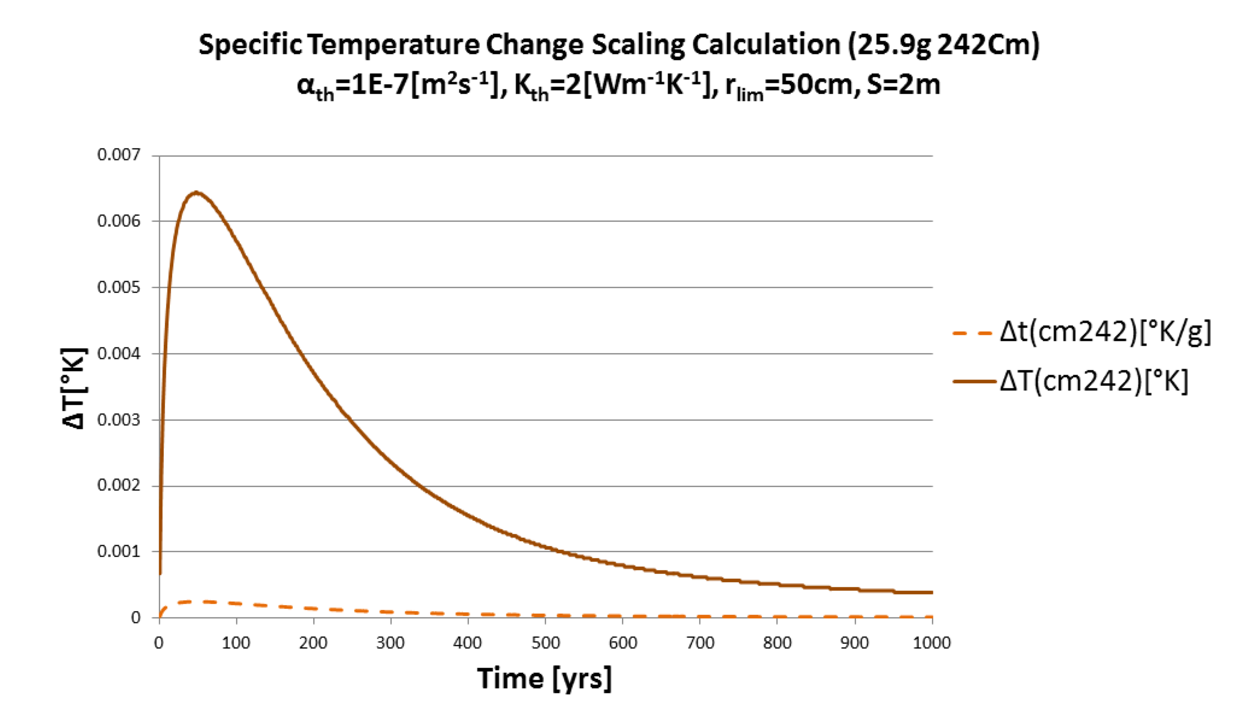
\includegraphics[width=\columnwidth]{images/CmScaling.eps}
\end{center}
\caption{As a demonstration of the calculation procedure, the temperature change 
  curve for one intial gram of $^{242}Cm$ and is scaled to represent $25.9g$, 
  approximately the $^{242}Cm$ inventory per MTHM in 51GWd burnum UOX PWR fuel. }
\label{fig:CmScaling}
\end{figure}

For an arbitrary waste stream 
composition, scaled curves calculated in this manner can be superimposed for 
each heat generating isotope to arrive at an approximate total temperature 
change at the calculation radius. 

To support this calculation in Cyder, a reference data set of temperature change 
curves, $\Delta t_i$, were calculated for high heat contributing isotopes. These 
curves were calclated as a function of specified repository spacing, $S$, heat 
limit radius, $r_{lim}$, and thermal paramters $\alpha_{th}$ and $K_{th}$. The 
total temperature change is the sum of the mass scaled curves,

\begin{align}
\Delta T &\sim \sum_{i\in H} m_i \Delta t_i(r,S,K_{th},\alpha_{th})
\intertext{where}
\Delta T &= \mbox{ total temperature change in waste }[^{\circ}K]\nonumber\\
H &= \mbox{ set of high heat isotopes }[-]\nonumber\\
m_i &= \mbox{ mass of isotope i  } [g]\nonumber\\
\Delta t_i(r,S,K_{th},\alpha_{th}) &= \mbox{ temperature change due to 1 g of i }[^{\circ}K]\nonumber
\label{superposition}
\end{align}

The use of this superposition is demonstrated in Figure 
\ref{fig:fakeArbitraryWF}.

\begin{figure}[ht!]
\begin{center}
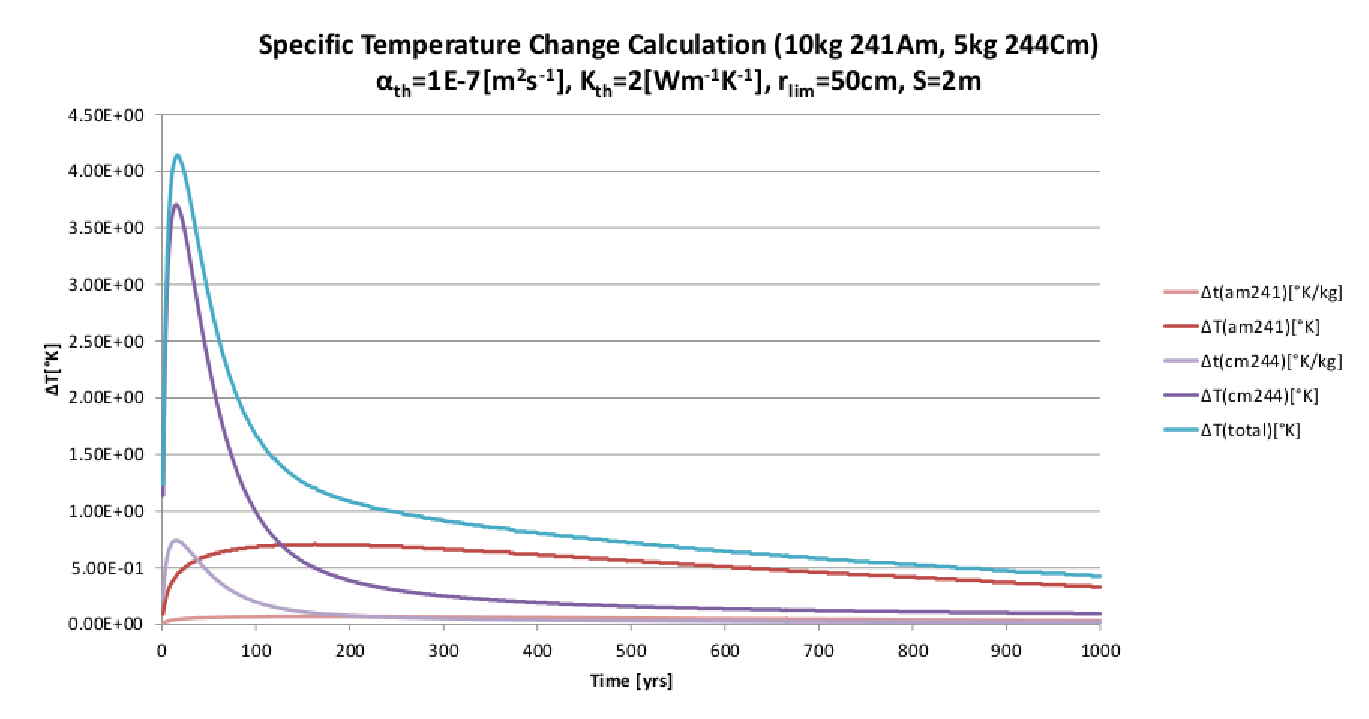
\includegraphics[width=\columnwidth]{images/fakeArbitraryWF.eps}
\end{center}
\caption{As a demonstration of the calculation procedure, scaled temperature change 
  curves for two isotopes are superimposed to achieve a total temperature 
change.}
\label{fig:fakeArbitraryWF}
\end{figure}


\begin{frame}[ctb!]
\frametitle{Specific Temperature Change Calculations}
\footnotesize{A reference data set of temperature change curves was calculated. 
Repeated runs of a detailed model over the range of values in Table 
\ref{tab:thermal_cases} determined Specific Temperature Change (STC) values over a range of thermal 
heat limit radii, $r_{lim}$, thermal diffusivity values, $\alpha_{th}$,
thermal conductivity values, $K_{th}$ and waste package spacings, $S$.

\begin{table}[ht!]
\centering
\footnotesize{
\begin{tabular}{|l|l|l|r|}
\multicolumn{4}{c}{\textbf{Thermal Cases}}\\
\hline
\textbf{Parameter} & \textbf{Symbol} & \textbf{Units} & \textbf{Value Range} \\
\hline
Diffusivity & $\alpha_{th}$ & $[m^2\cdot s^{-1}]$ & $1.0\times10^{-7}-3.0\times10^{-6}$\\
\hline
Conductivity & $K_{th}$     & $[W\cdot m^{-1} \cdot K^{-1}]$ & $0.1 - 4.5$ \\
\hline
Spacing & $S$ & $[m]$ & 2, 5, 10, 15, 20, 25, 50 \\
\hline
Radius & $r_{lim}$ & $[m]$ & 0.1, 0.25, 0.5, 1, 2, 5 \\
\hline
Isotope & $i$ & $[-]$ & $^{241,243}Am,$  \\
        & & & $^{242,243,244,245,246}Cm,$  \\
        & & & $^{238,240,241,242}Pu$  \\
        & & & $^{134,135,137}Cs$  \\
        & & & $^{90}Sr$  \\
\hline
\end{tabular}
\caption{A thermal reference dataset of \gls{STC} values as a function of each of these parameters was generated by repeated parameterized runs of the LLNL 
MathCAD model\cite{greenberg_application_2012, greenberg_investigations_2012}.}
\label{tab:thermal_cases}
}
\end{table}


}
\end{frame}


\begin{frame}[ctb!]
\frametitle{LLNL UFD MathCAD Model}
\footnotesize{
The analytic model used to populate the reference dataset was created at 
LLNL for the UFD campaign \cite{hardin_generic_2011, 
greenberg_investigations_2012, greenberg_application_2012}. It employs an 
analytic model from Carslaw and Jaeger and is \textbf{implemented in MathCAD}
\cite{carslaw_conduction_1959, ptc_mathcad_2010}.  The integral solver in the 
MathCAD toolset is the primary calculation engine for the analytic MathCAD 
thermal model, which relies on superposition of point, finite-line, and line 
source integral solutions.  
}
\end{frame}


\begin{frame}[ctb!]
\frametitle{Scaling Demonstration}
\footnotesize{

\begin{figure}[h!]
\begin{center}
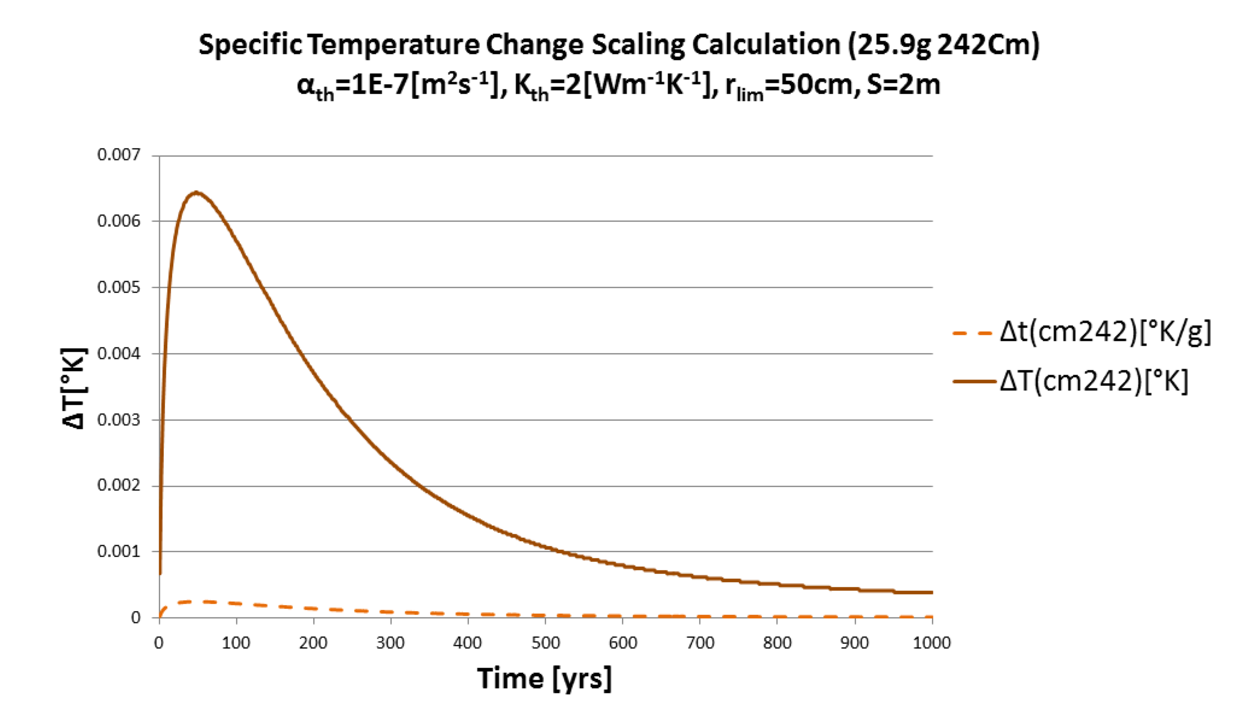
\includegraphics[width=\linewidth]{./images/CmScaling.eps}
\end{center}
\caption{As a demonstration of the calculation procedure, the temperature change 
  curve for one initial gram of $^{242}Cm$ and is scaled to represent $25.9g$, 
  approximately the $^{242}Cm$ inventory per MTHM in 51GWd burnup UOX PWR fuel. }
\label{fig:CmScaling}
\end{figure}
}
\end{frame}

\begin{frame}
\frametitle{Superposition Concept}
\footnotesize{

The supporting database was limited to some primary heat contributing isotopes 
present in traditional spent nuclear fuel, $H$, 
such that the superposition in equation \eqref{superposition} becomes 
\begin{align}
\Delta T (r_{lim},S,K_{th},\alpha_{th})&\sim \sum_{i\in H} m_i \Delta t_i(r_{lim},S,K_{th},\alpha_{th})
\label{superposition_approx}
\intertext{where}
H &= \mbox{ set of high heat isotopes }[-]\nonumber\\
S &= \mbox{ uniform waste package spacing } [m]\nonumber\\
K_{th} &= \mbox{ thermal conductivity } [W\cdot m^{-1}\cdot K^{-1}]\nonumber\\
\alpha_{th} &= \mbox{ thermal diffusivity } [m^2\cdot s^{-1}]\nonumber\\
\end{align}
}
\end{frame}


\begin{frame}
\frametitle{Superposition Demonstration}
\footnotesize{

\begin{figure}[ht!]
\begin{center}
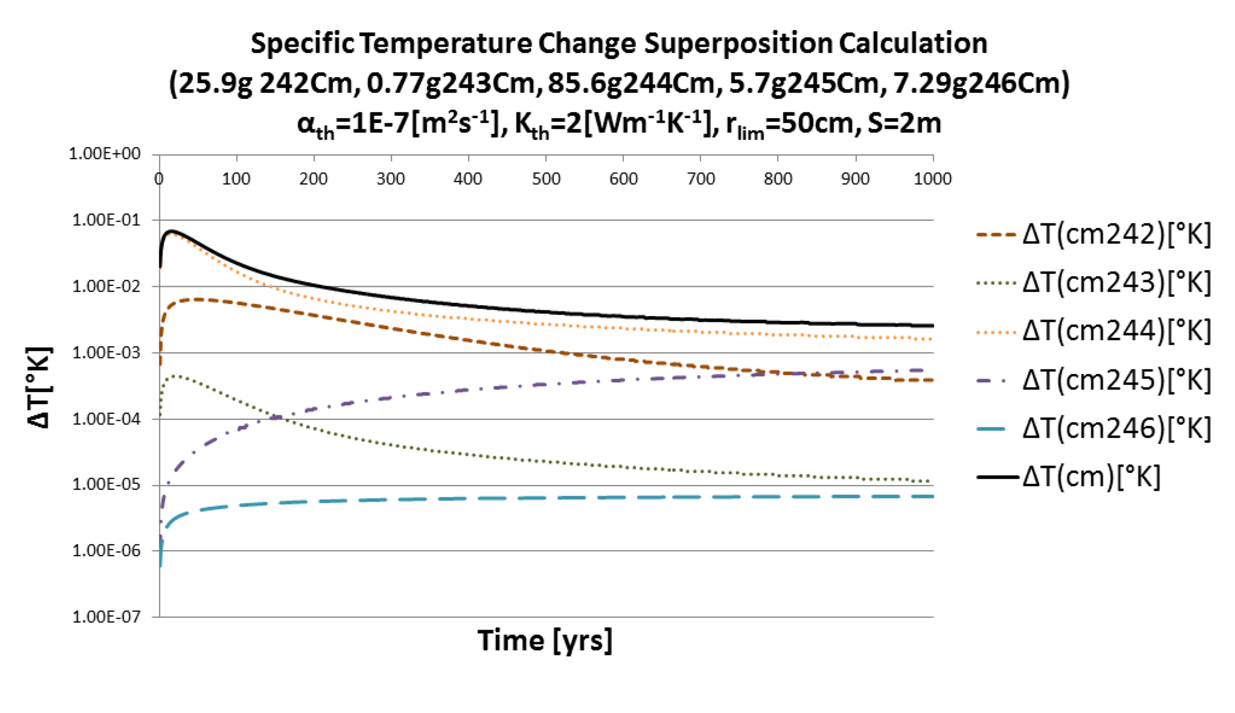
\includegraphics[width=\columnwidth]{./images/CmSuperposition.eps}
\end{center}
\caption{As a demonstration of the calculation procedure, scaled temperature change 
  curves for five curium isotopes are superimposed to achieve a total temperature 
change (note log scale).}
\label{fig:CmSuperposition}
\end{figure}

}
\end{frame}




\section{Demonstration}
\subsection{Base Cases}

\begin{frame}[ctb!]
  \frametitle{Thermal Base Case Demonstration}
  \footnotesize{
\begin{figure}[htp!]
\begin{center}
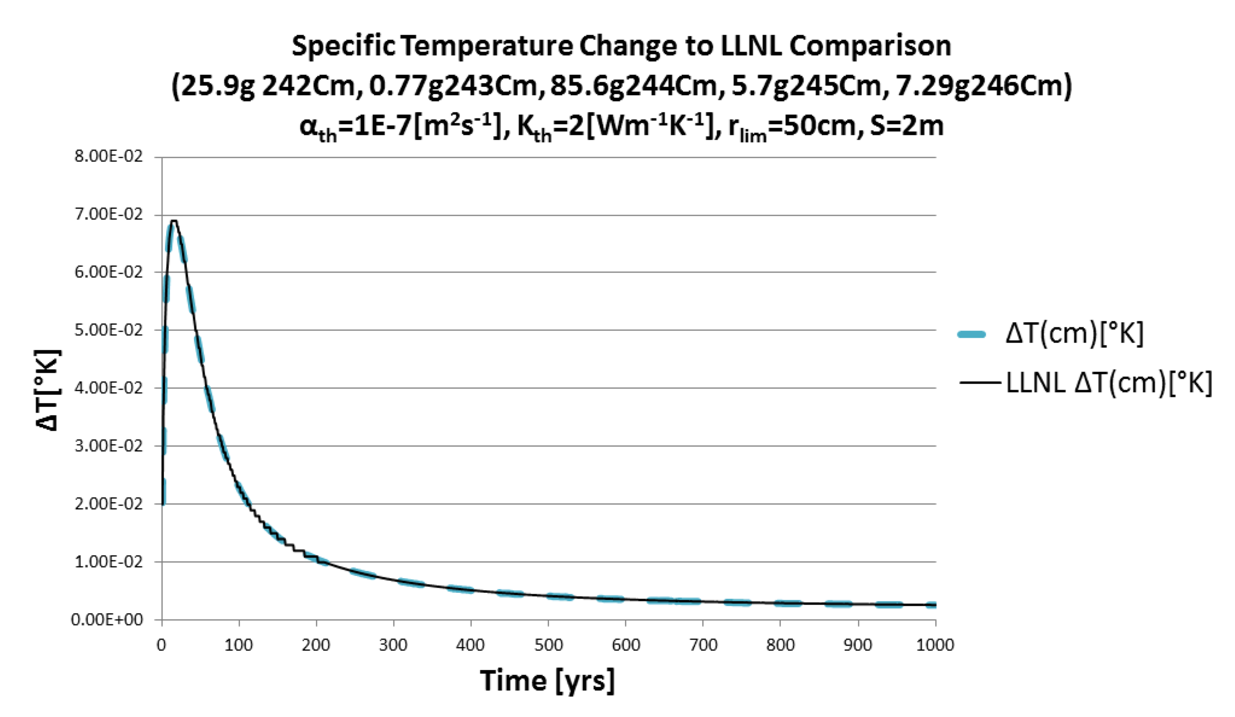
\includegraphics[width=\columnwidth]{./thermal_demonstration/CmValidation.eps}
\end{center}
\caption{This comparison of STC calculated thermal response from $Cm$ 
inventory per MTHM in 51GWd burnup UOX PWR fuel 
demonstrates an average error of 1.1\% and a 
maximum error of 4.4\%}
\label{fig:CmValidation}
\end{figure}
  }
\end{frame}


\begin{frame}[ctb!]
  \frametitle{Thermal Base Case Demonstration}
\begin{figure}[htp!]
\begin{center}
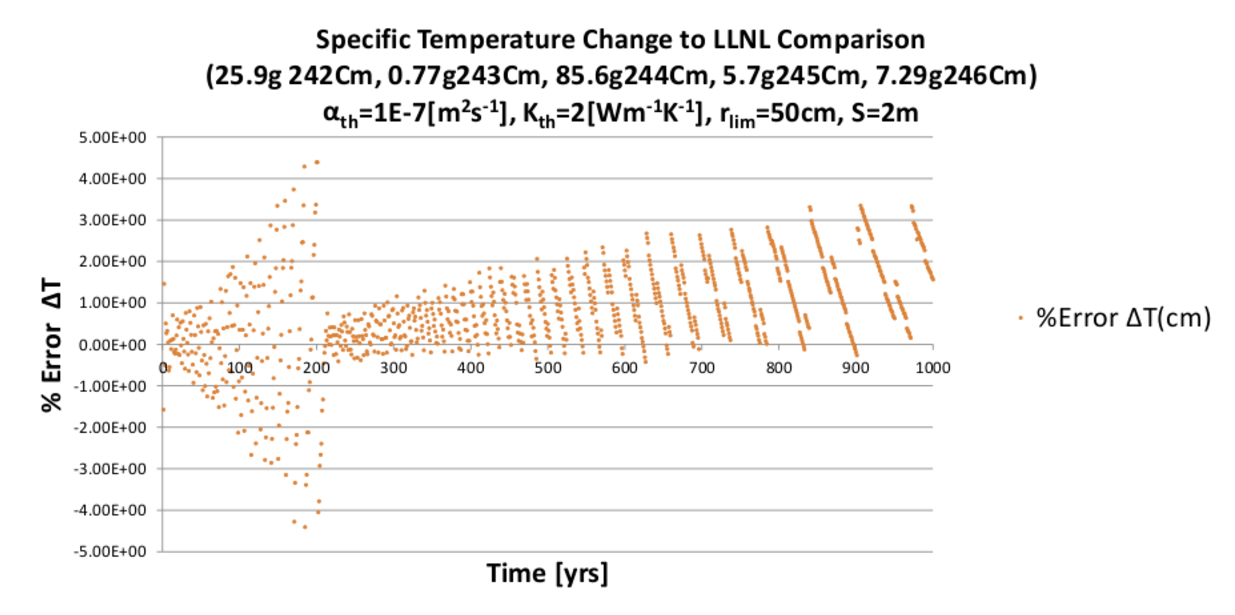
\includegraphics[width=\columnwidth]{./thermal_demonstration/CmPercentError.eps}
\end{center}
\caption{Percent error between the semi-analytic model from LLNL and the STC 
calculated thermal response from $Cm$ inventory per MTHM in 51GWd burnup UOX 
PWR fuel demonstrates a maximum percent error of 4.4\%.}
\label{fig:CmPercentError}
\end{figure}
\end{frame}


\subsection{Validation Cases}



\begin{frame}[ctb!]
\frametitle{LLNL Model Waste Package Spacing Sensitivity}
\footnotesize{
\begin{figure}[htbp!]
\begin{center}
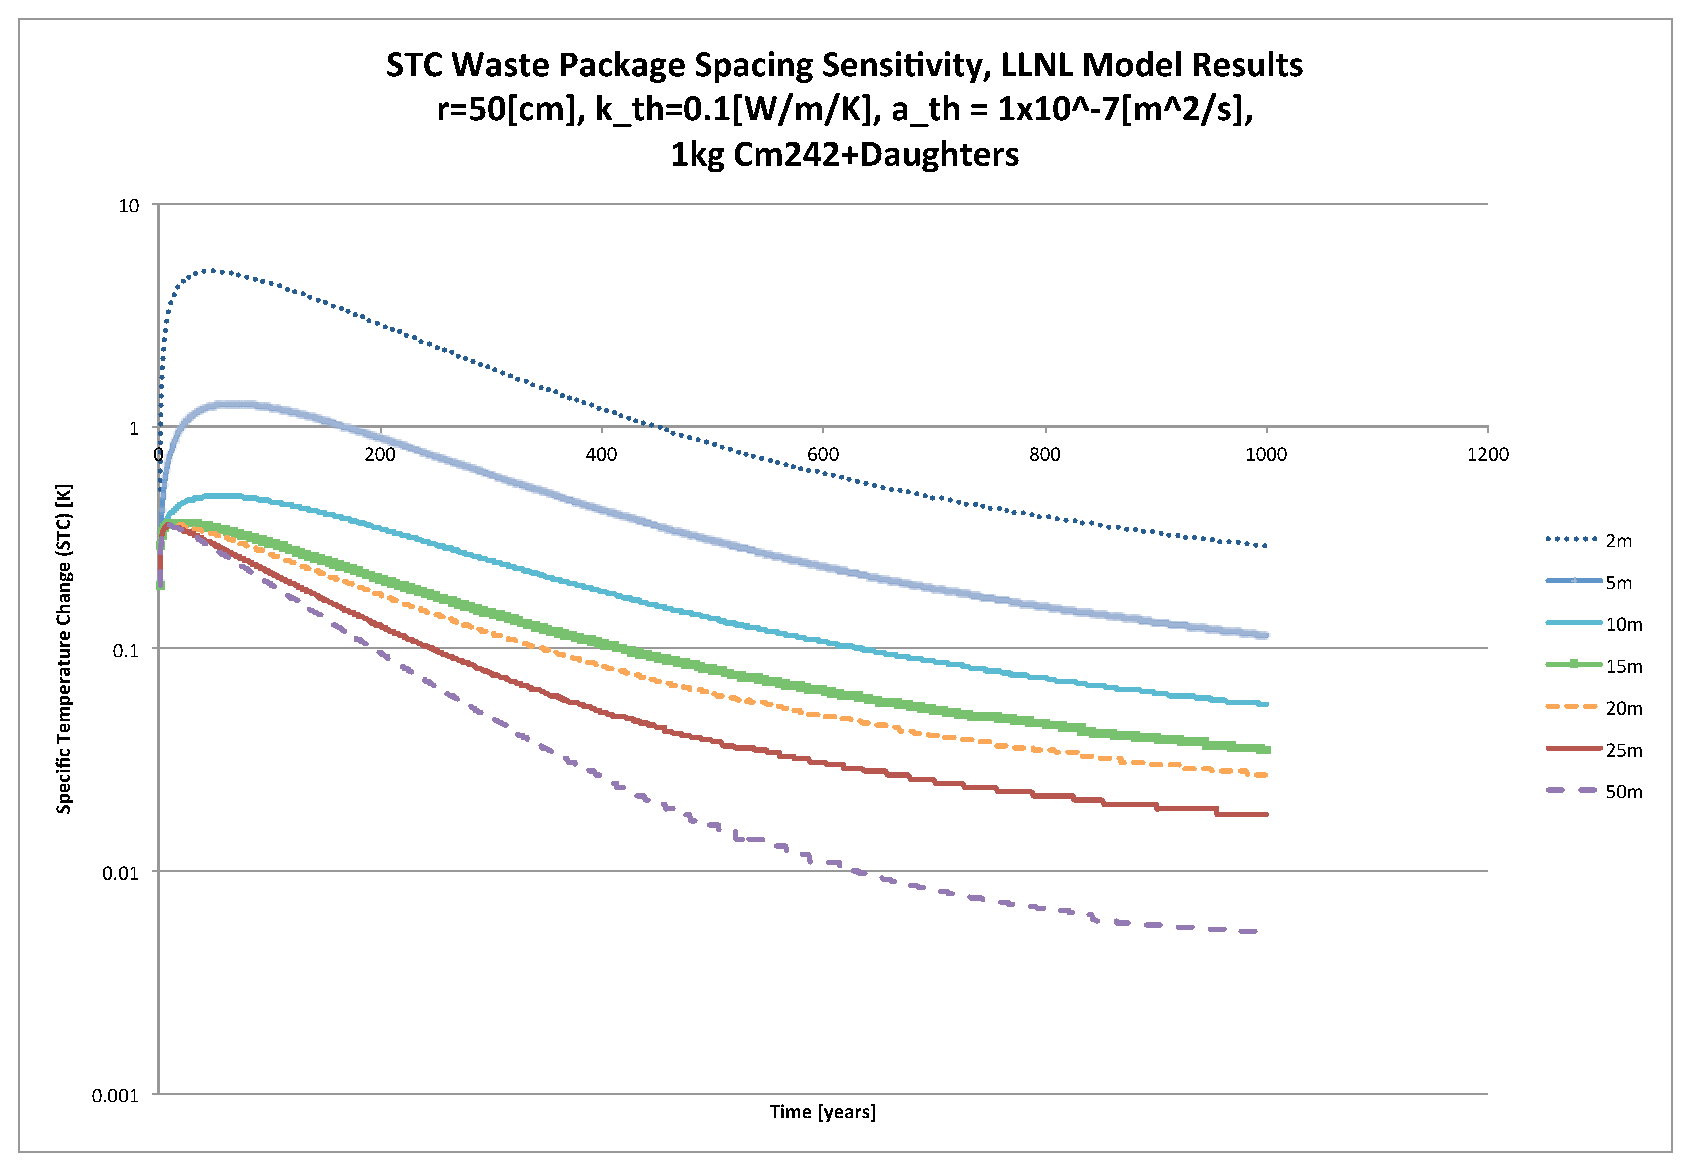
\includegraphics[height=0.7\textheight]{./thermal_demonstration/spacing/Cm242spacing_sens.eps}
\end{center}
\caption[$K_{th}$ Sensitivity to $s$]{Increased waste package 
spacing decreases areal thermal energy deposition 
(here represented by STC) in the near field (here $r_{calc} = 0.5m$).}
\label{fig:Cm242spacing_sens}
\end{figure}
}
\end{frame}


\begin{frame}[ctb!]
\frametitle{LLNL Model Limiting Radius Sensitivity}
\footnotesize{
\begin{figure}[htbp!]
\begin{center}
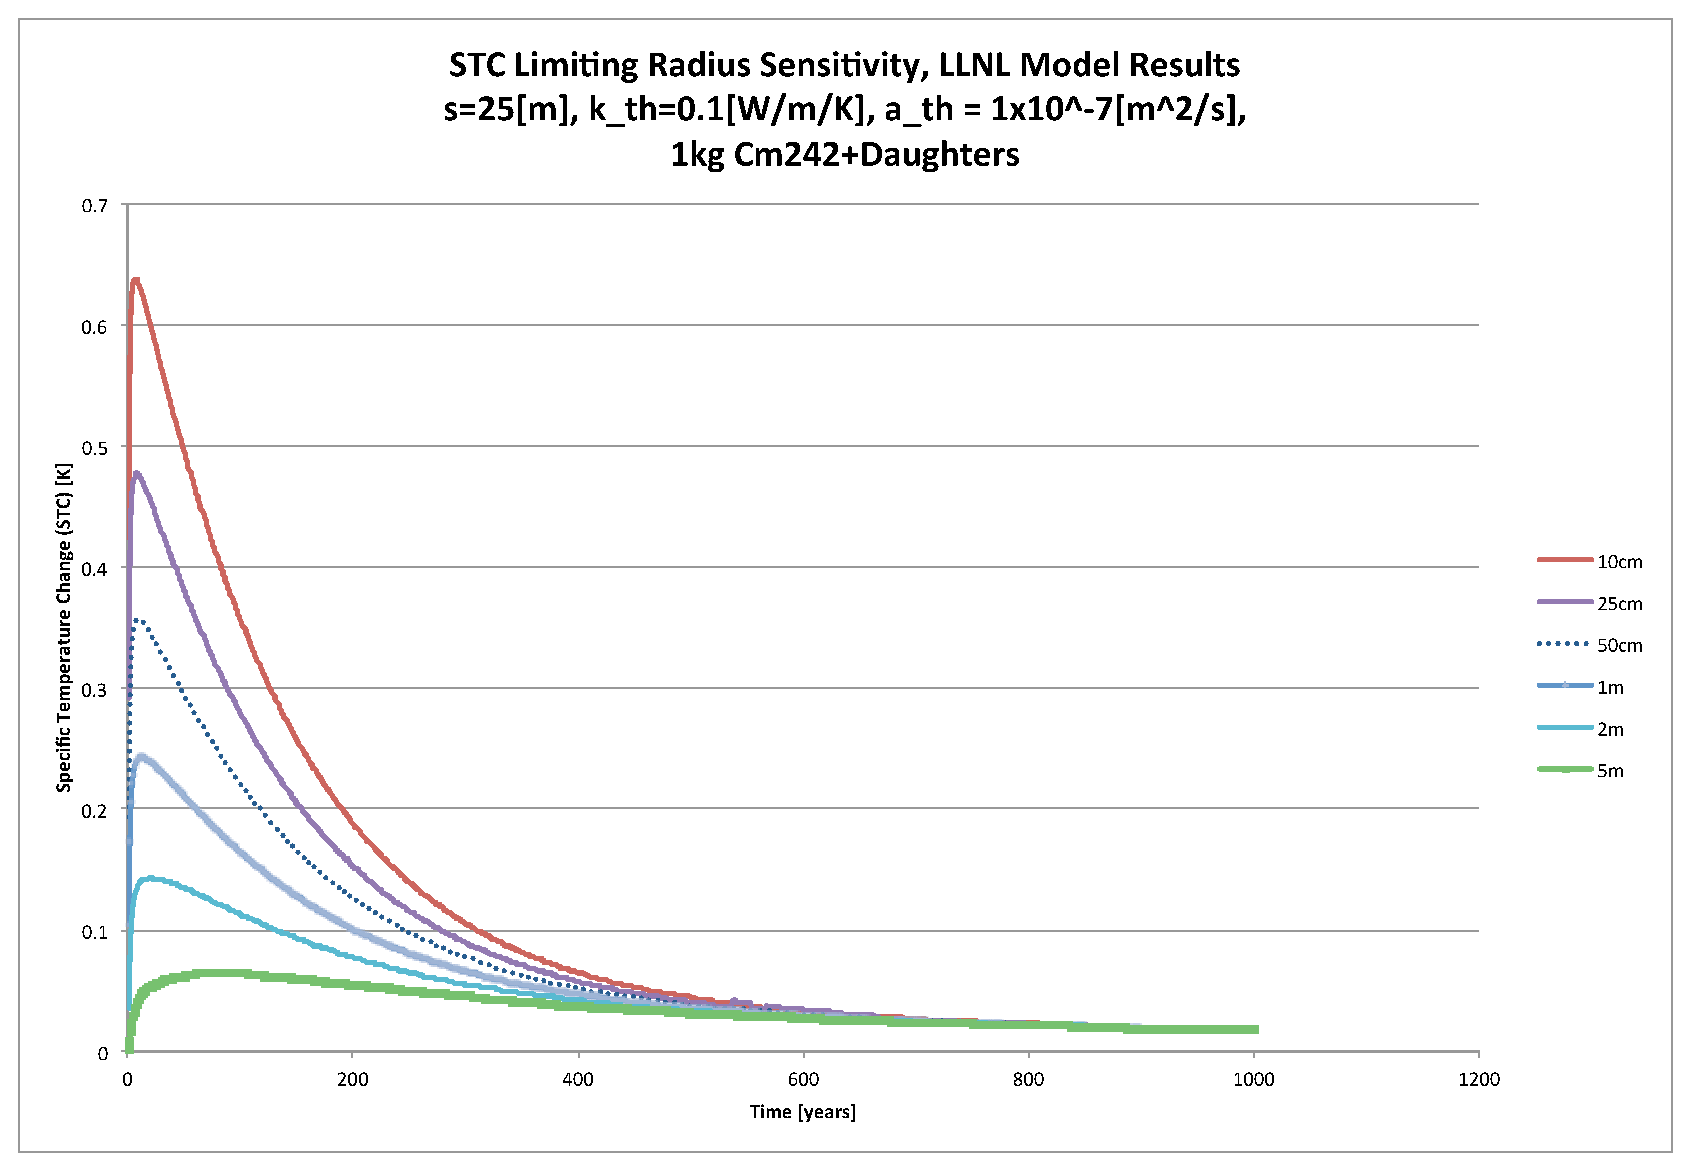
\includegraphics[height=0.7\textheight]{./thermal_demonstration/spacing/Cm242r_lim_sens.eps}
\end{center}
\caption[$K_{th}$ Sensitivity to $r_{lim}$]{
The location of the limiting radius has a strong effect on the 
waste package loading limit, for a fixed limiting temperature.} 
\label{fig:Cm242r_lim_sens}
\end{figure}
}
\end{frame}

\begin{frame}[ctb!]
\frametitle{Cyder Spacing and Limiting Radius Sensitivity}
\footnotesize{
\begin{figure}[htbp!]
\begin{center}
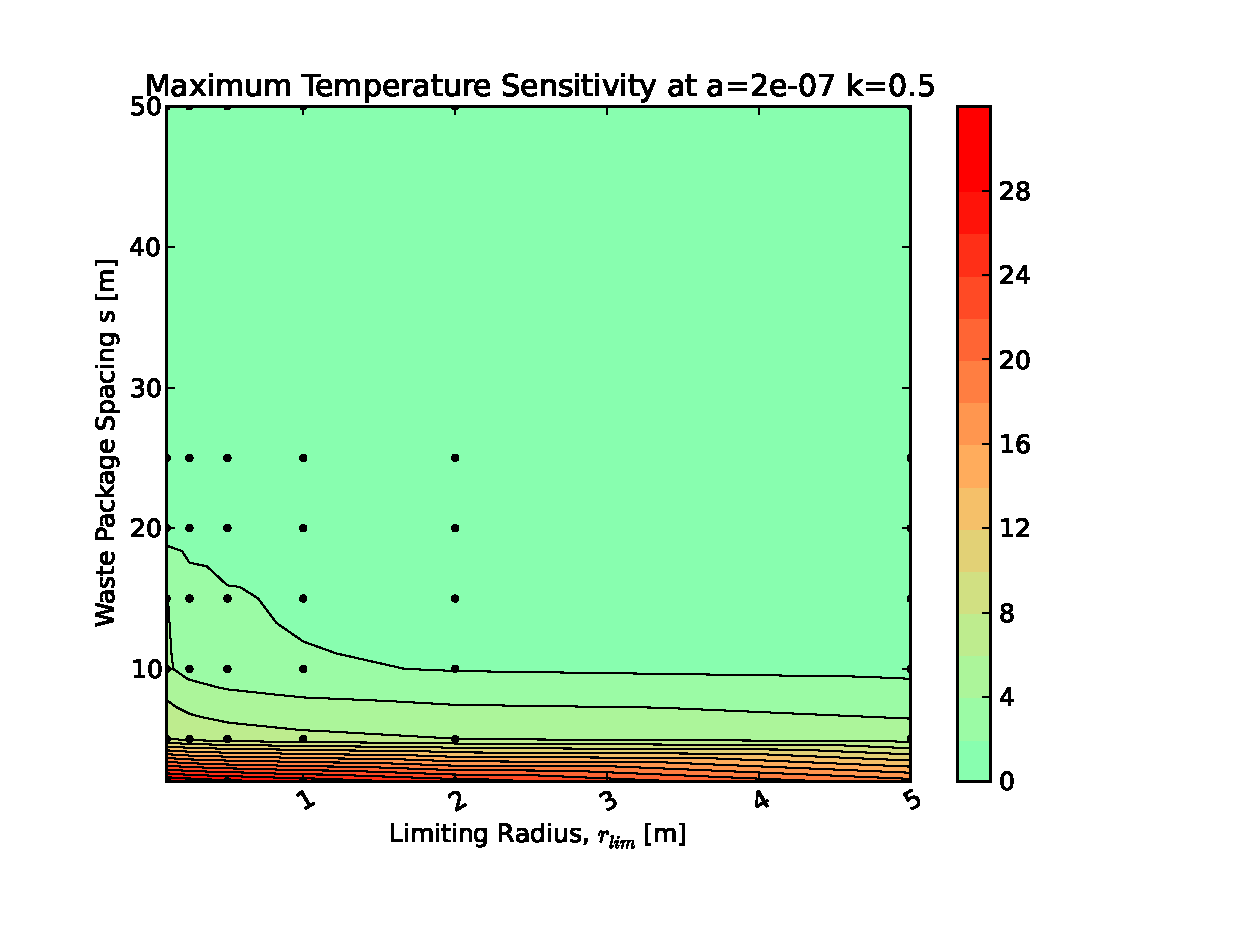
\includegraphics[height=0.7\textheight]{./thermal_demonstration/spacing/rs.eps}
\end{center}
\caption[$\alpha_{th}$ vs. $r_{lim}$ Sensitivity in Cyder]{Cyder results agree with 
those of the LLNL model. The importance of the limiting radius decreases with 
increased $S$. The above example thermal profile results from 10kg of 
$^{242}Cm$}
\label{fig:rs}
\end{figure}
}
\end{frame}



\begin{frame}[ctb!]
\frametitle{LLNL Model Thermal Conductivity Sensitivity}
\begin{figure}[htbp!]
\begin{center}
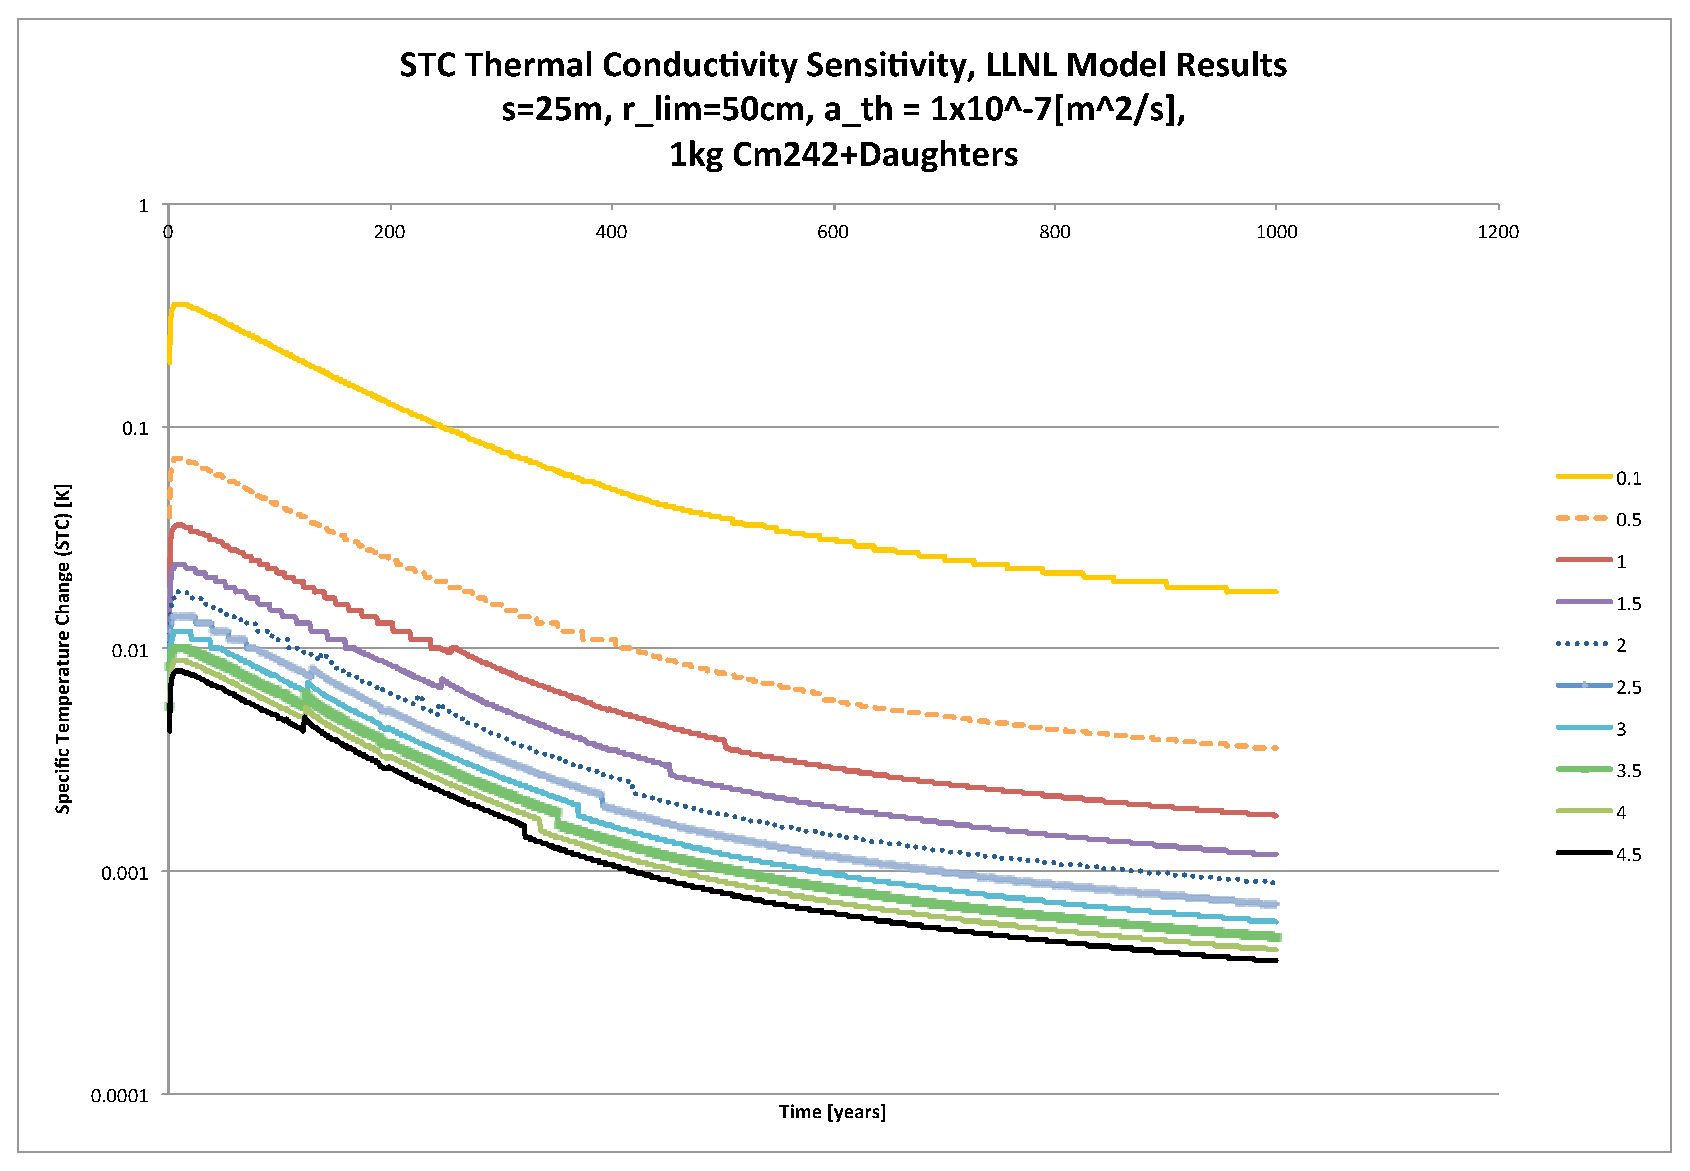
\includegraphics[height=0.7\textheight]{./thermal_demonstration/conductivity/Cm242kth_alpha_low.eps}
\end{center}
\caption[$K_{th}$ Sensitivity for Low $\alpha_{th}$ in LLNL Model]{
By varying the thermal conductivity of the repository model from 0.1 to 4.5 
$[W\cdot m^{-1} \cdot K^{-1}]$, this sensitivity analysis succeeds in capturing 
the domain of thermal conductivities witnessed in high thermal conductivity 
salt deposits as well as low thermal conductivity clays.}
\label{fig:Cm242Kth_alpha_low}
\end{figure}

\end{frame}


\begin{frame}[ctb!]
\frametitle{Cyder Thermal Conductivity and Limiting Radius Sensitivity}


\begin{figure}[htbp!]
\begin{center}
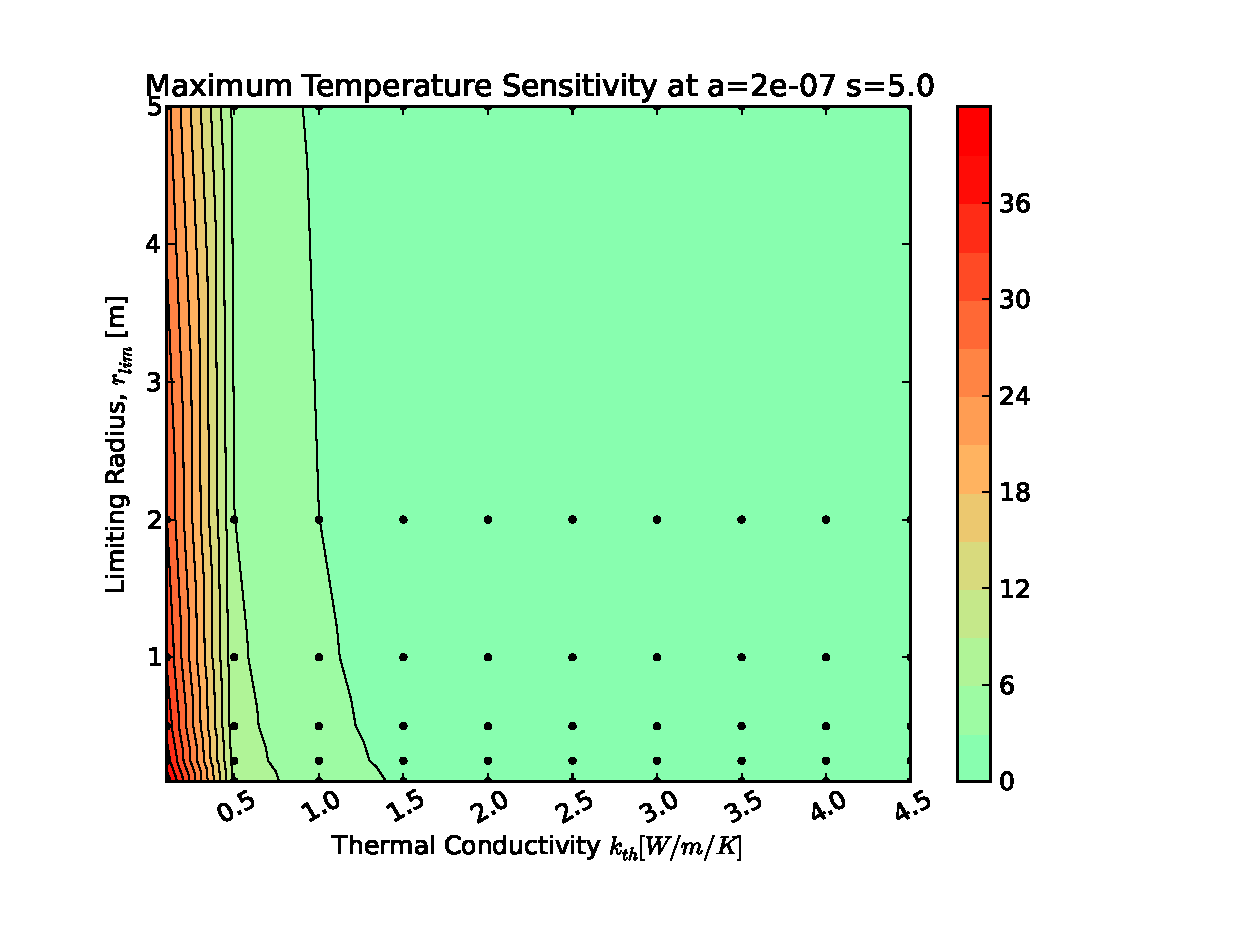
\includegraphics[height=0.7\textheight]{./thermal_demonstration/conductivity/kr.eps}
\end{center}
\caption[$K_{th}$ vs. $r_{lim}$ Sensitivity in Cyder]
{
Increased thermal conductivity of a medium decreases thermal energy deposition 
in the near field. Additionally, analysis with the \Cyder STC database 
demonstrates the way in which the importance of spacing and the importance of 
the limiting radius decrease with increasing $K_{th}$.
The above example thermal profile results from 10kg of 
$^{242}Cm$}
\label{fig:kr}
\end{figure}
\end{frame}

\begin{frame}[ctb!]
\frametitle{Cyder Thermal Conductivity and Limiting Radius Sensitivity}

\begin{figure}[htbp!]
\begin{center}
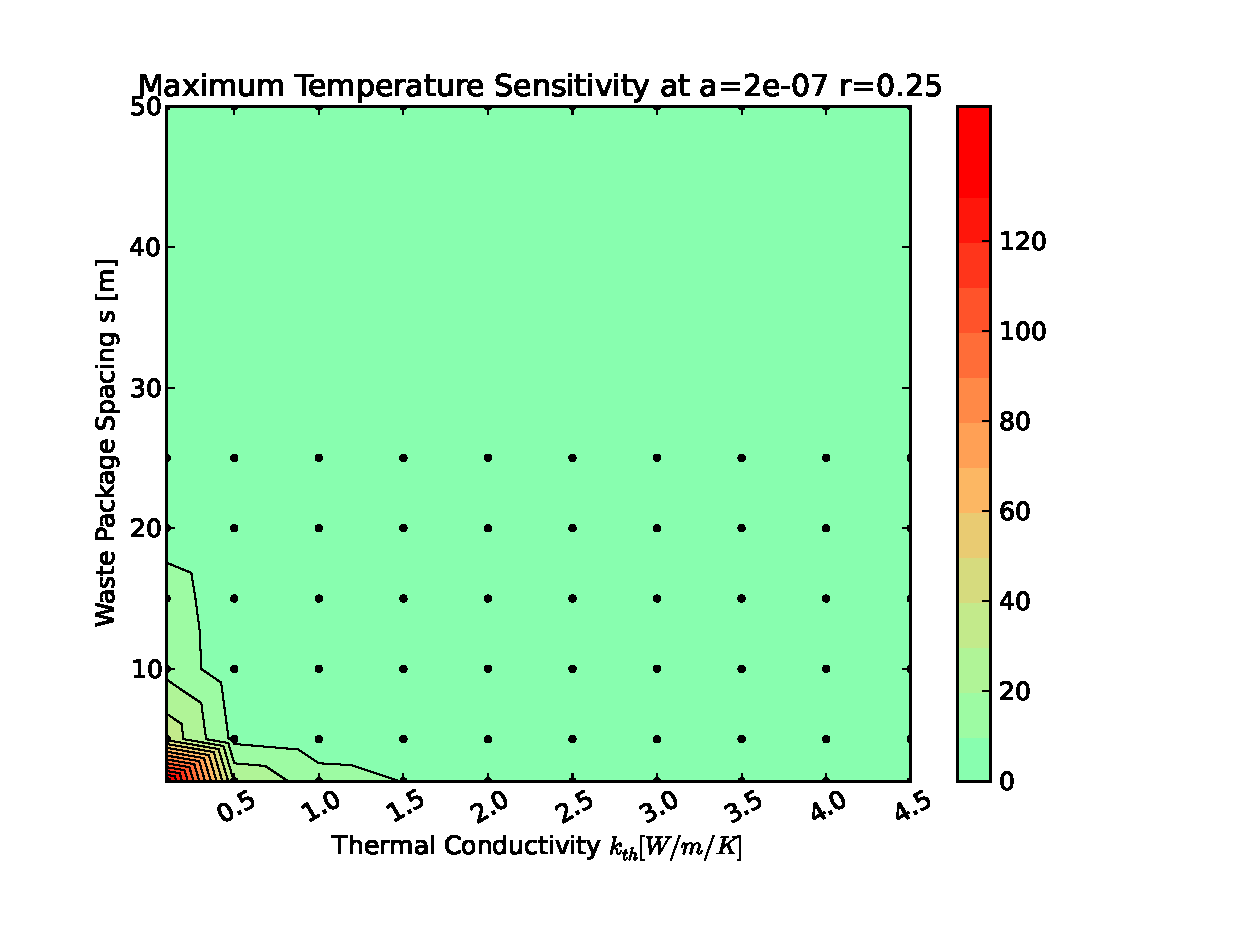
\includegraphics[height=0.7\textheight]{./thermal_demonstration/conductivity/ks.eps}
\end{center}
\caption[$K_{th}$ vs. Waste Package Spacing Sensitivity in Cyder]{
The combined effect of waste package spacing and $K_{th}$ is strong. The above example thermal profile results from 10kg of 
$^{242}Cm$}
\label{fig:ks}
\end{figure}
\end{frame}




\begin{frame}[ctb!]
\frametitle{LLNL Model Thermal Diffusivity Sensitivity}
\footnotesize{

\begin{figure}[htbp!]
\begin{center}
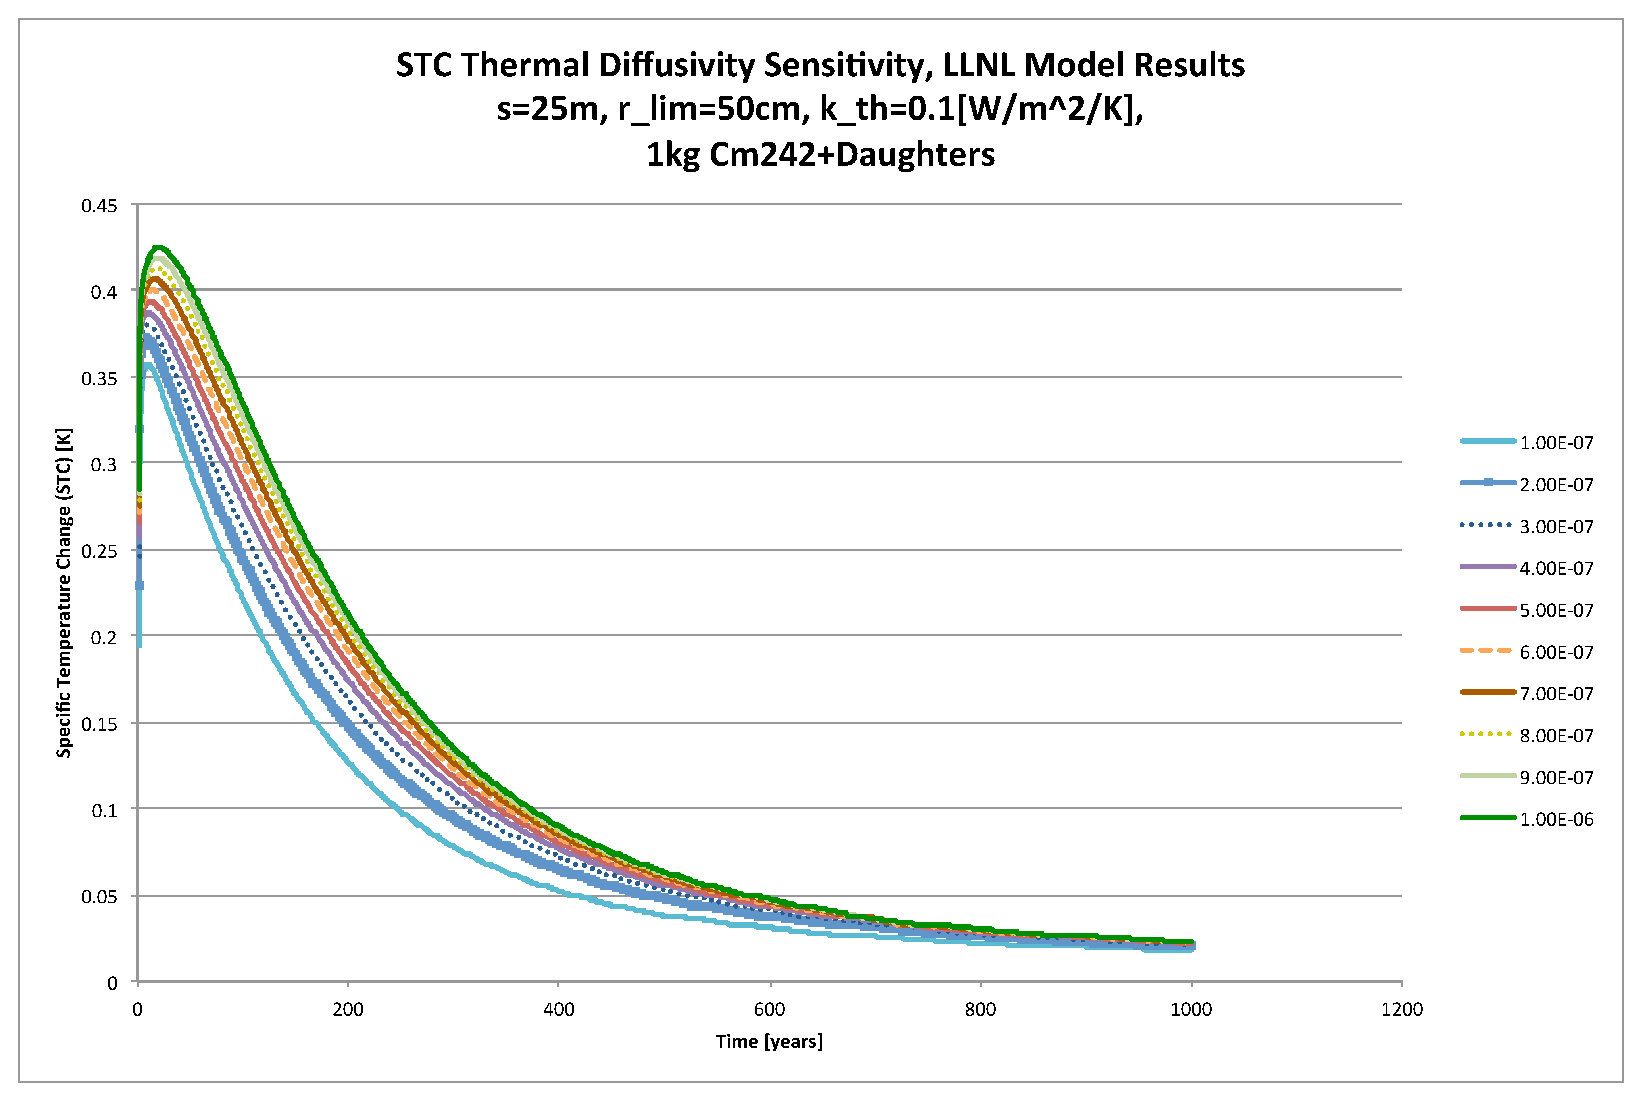
\includegraphics[height=0.7\textheight]{./thermal_demonstration/diffusivity/Cm242alpha_kth_low.eps}
\end{center}
\caption[$K_{th}$ Sensitivity to $\alpha_{th}$ for $k_{th}$]{
By varying the thermal diffusivity of the disposal system from $0.1-3\times 
10^{-6} [m^2\cdot s^{-1}]$, this sensitivity analysis succeeds in capturing the domain of 
thermal diffusivities witnessed in high thermal diffusivity salt deposits as 
well as low thermal diffusivity clays.}
\label{fig:Cm242alpha_kth_low}
\end{figure}
}
\end{frame}


\begin{frame}[ctb!]
\frametitle{Cyder Thermal Diffusivity and Conductivity Sensitivity}
\footnotesize{
\begin{figure}[htbp!]
\begin{center}
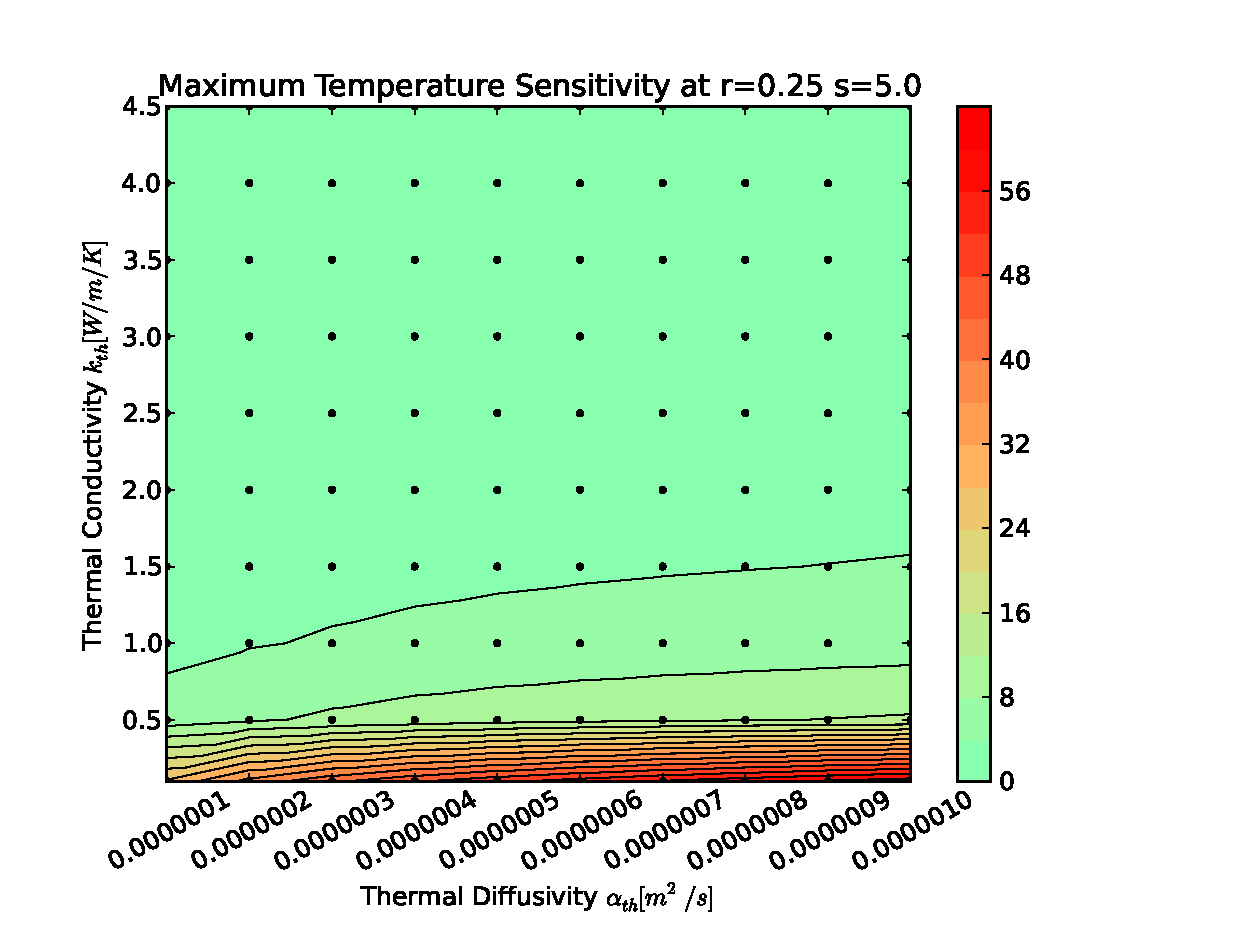
\includegraphics[height=0.7\textheight]{./thermal_demonstration/diffusivity/ak.eps}
\caption[$\alpha_{th}$ vs. $K_{th}$ Sensitivity in Cyder]{Cyder trends agree
with those of the LLNL model, in which increased thermal diffusivity results in 
increased thermal depsoition in the near field. The above example thermal 
profile results from 10kg of $^{242}Cm$.} 
\label{fig:ar}
\end{center}
\end{figure}
}
\end{frame}

\begin{frame}[ctb!]
\frametitle{Cyder Thermal Diffusivity and Limiting Radius Sensitivity}
\footnotesize{
\begin{figure}[htbp!]
\begin{center}
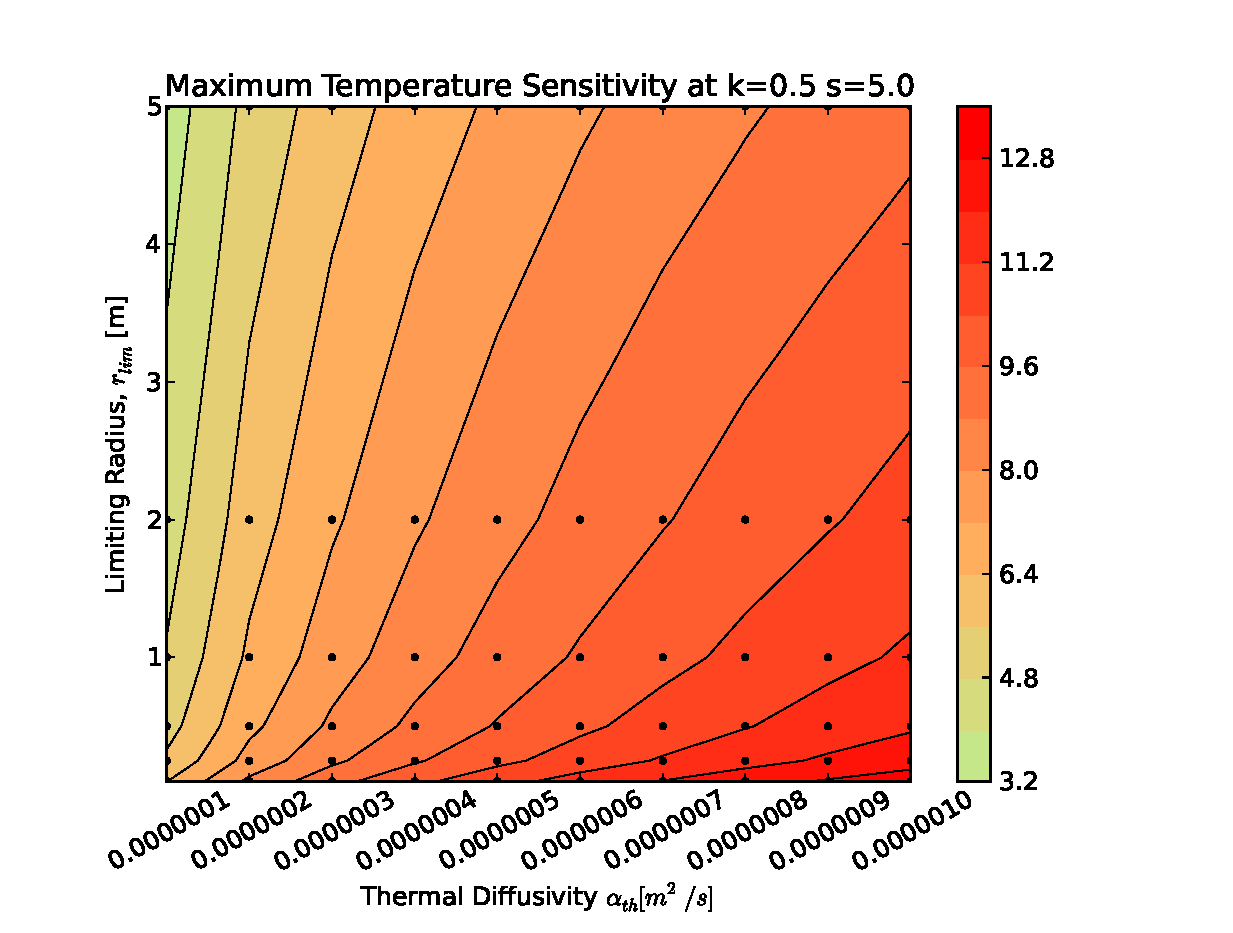
\includegraphics[height=0.7\textheight]{./thermal_demonstration/diffusivity/ar.eps}
\end{center}
\caption[$\alpha_{th}$ vs. $r_{lim}$ Sensitivity in Cyder]
{Cyder trends agree with 
those of the LLNL model. The importance of the limiting radius decreases with 
increased $\alpha_{th}$. The above example thermal profile results from 10kg of 
$^{242}Cm$}
\label{fig:ak}
\end{figure}
}
\end{frame}




\begin{frame}[c]
  \frametitle{Acknowledgements}
This work is supported by the U.S. Department of Energy, Basic Energy Sciences, 
Office of Nuclear Energy, under contract \# DE-AC02-06CH11357.
\end{frame}


\begin{frame}[allowframebreaks]
  \frametitle{References}
  \bibliographystyle{plain}
  {\footnotesize \bibliography{ans_2013_therm}}
\end{frame}

\subsubsection{Supporting Thermal Response Dataset}
To support this calculation in Cyder, a reference data set of temperature change 
curves was calculated. Repeated runs of a detailed analytic model over the range of values in Table 
\ref{tab:thermal_cases} determined \gls{STC} values over a range of thermal 
heat limit radii, $r_{lim}$, thermal diffusivity values, $\alpha_{th}$,
thermal conductivity values, $K_{th}$ and waste package spacings, $S$. Linear 
interpolation across the discrete parameter space provides a simple thermal 
reference dataset for use in Cyder.

\begin{table}[ht!]
\centering
\footnotesize{
\begin{tabular}{|l|l|l|r|}
\multicolumn{4}{c}{\textbf{Thermal Cases}}\\
\hline
\textbf{Parameter} & \textbf{Symbol} & \textbf{Units} & \textbf{Value Range} \\
\hline
Diffusivity & $\alpha_{th}$ & $[m^2\cdot s^{-1}]$ & $1.0\times10^{-7}-3.0\times10^{-6}$\\
\hline
Conductivity & $K_{th}$     & $[W\cdot m^{-1} \cdot K^{-1}]$ & $0.1 - 4.5$ \\
\hline
Spacing & $S$ & $[m]$ & 2, 5, 10, 15, 20, 25, 50 \\
\hline
Radius & $r_{lim}$ & $[m]$ & 0.1, 0.25, 0.5, 1, 2, 5 \\
\hline
Isotope & $i$ & $[-]$ & $^{241,243}Am,$  \\
        & & & $^{242,243,244,245,246}Cm,$  \\
        & & & $^{238,240,241,242}Pu$  \\
        & & & $^{134,135,137}Cs$  \\
        & & & $^{90}Sr$  \\
\hline
\end{tabular}
\caption{A thermal reference dataset of \gls{STC} values as a function of each of these parameters was generated by repeated parameterized runs of the LLNL 
MathCAD model\cite{greenberg_application_2012, greenberg_investigations_2012}.}
\label{tab:thermal_cases}
}
\end{table}



The analytic model used to populate the reference dataset was created at 
\gls{LLNL} for the \gls{UFD} campaign. In this tool, heat limited thermal 
response is calculated analytically for each geology, for many waste package 
loading densities, and for many fuel cycle options \cite{hardin_generic_2011, 
greenberg_investigations_2012, greenberg_application_2012}. It employs an 
analytic model from Carslaw and Jaeger and is implemented in MathCAD 
\cite{carslaw_conduction_1959, ptc_mathcad_2010}.  The integral solver in the 
MathCAD toolset is the primary calculation engine for the analytic MathCAD 
thermal model, which relies on superposition of point, finite-line, and line 
source integral solutions.  

%The transient state of the temperature at the calculation radius is found with a convolution of the transient far field solution with the steady state near field solution.  The process is then iterated with a one year resolution in order to arrive at a temperature evolution over the lifetime of the repository. 
%
%In a two dimensional grid of waste packages, the central package is represented by the finite line solution

Figure \ref{fig:CmScaling} demonstrates the scaling of an STC curve according to 
equation \eqref{STC} to represent the heat from $25.9g$ of initial $^{242}Cm$ using 
the reference data set. 

\begin{figure}[h!]
\begin{center}
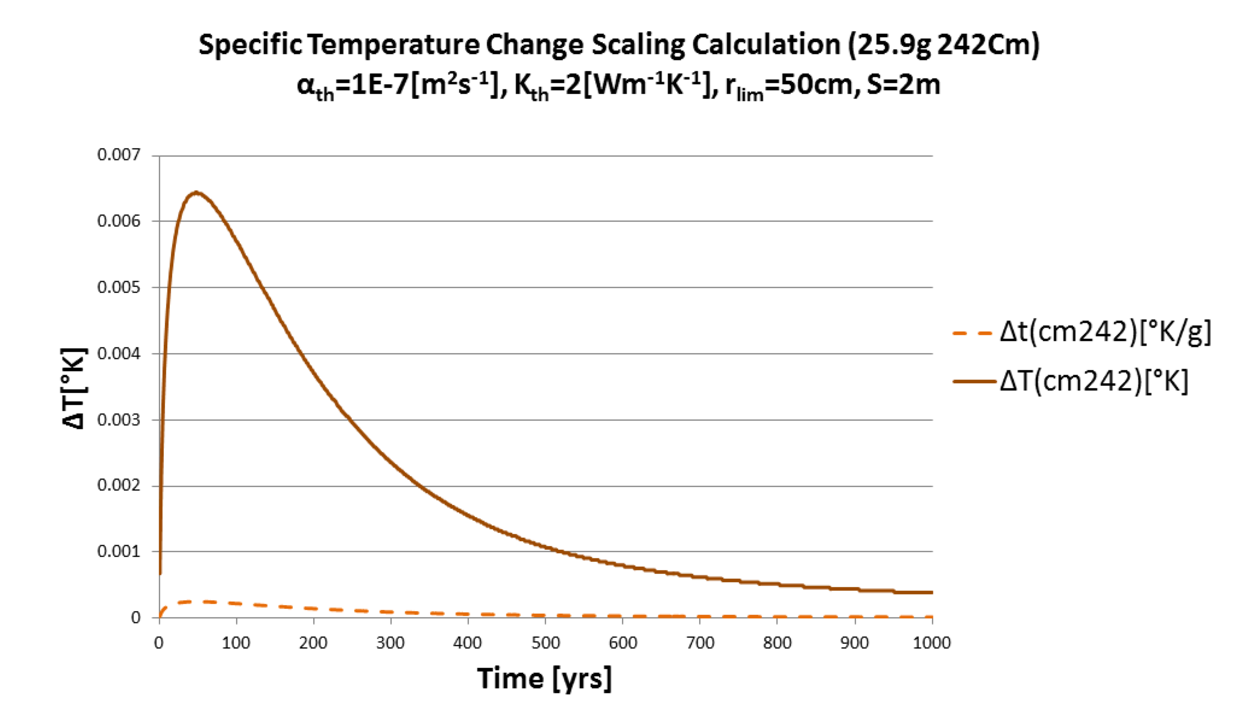
\includegraphics[width=\columnwidth]{images/CmScaling.eps}
\end{center}
\caption{As a demonstration of the calculation procedure, the temperature change 
  curve for one initial gram of $^{242}Cm$ and is scaled to represent $25.9g$, 
  approximately the $^{242}Cm$ inventory per MTHM in 51GWd burnup UOX PWR fuel. }
\label{fig:CmScaling}
\end{figure}


The supporting database was limited to  high heat contributing isotopes, $H$, 
such that the superposition in equation \eqref{superposition} becomes 

\begin{align}
\Delta T (r_{lim},S,K_{th},\alpha_{th})&\sim \sum_{i\in H} m_i \Delta t_i(r_{lim},S,K_{th},\alpha_{th})
\label{superposition_approx}
\intertext{where}
H &= \mbox{ set of high heat isotopes }[-]\nonumber\\
S &= \mbox{ uniform waste package spacing } [m]\nonumber\\
K_{th} &= \mbox{ thermal conductivity } [W\cdot m^{-1}\cdot K^{-1}]\nonumber\\
\alpha_{th} &= \mbox{ thermal diffusivity } [m^2\cdot s^{-1}]\nonumber\\
\end{align}

The use of this superposition is demonstrated in Figure 
\ref{fig:CmSuperposition}.

\begin{figure}[ht!]
\begin{center}
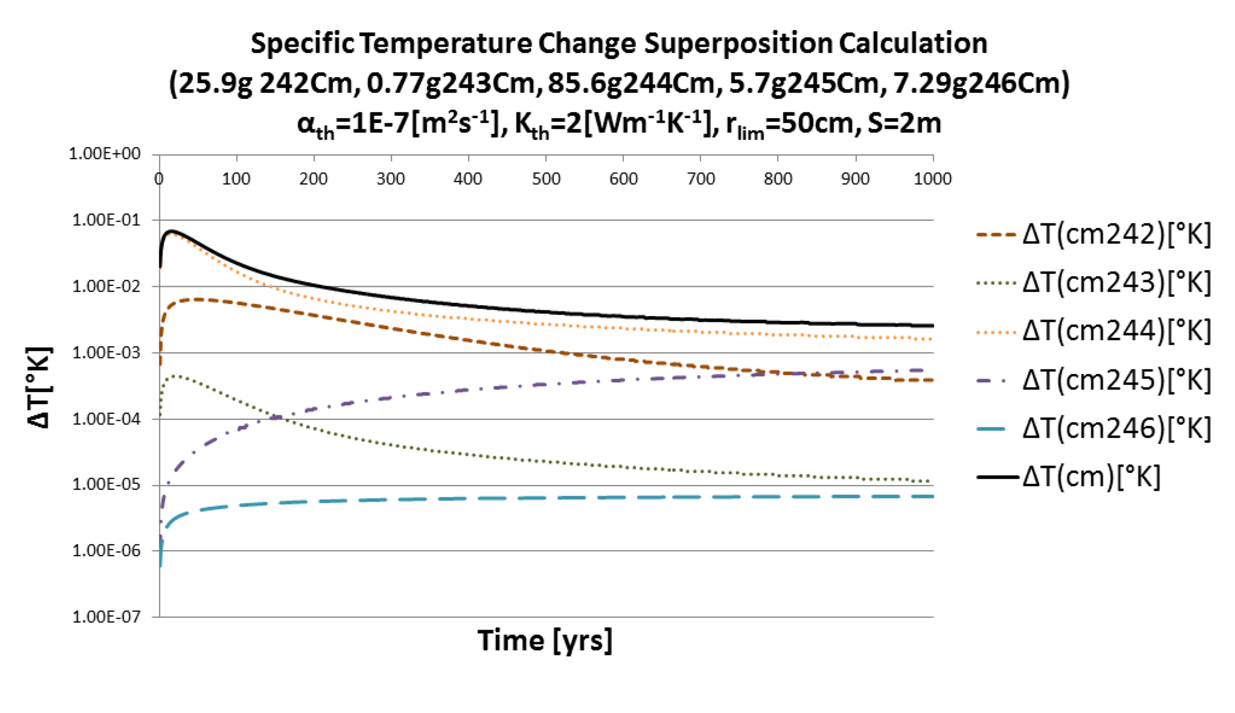
\includegraphics[width=\columnwidth]{images/CmSuperposition.eps}
\end{center}
\caption{As a demonstration of the calculation procedure, scaled temperature change 
  curves for two isotopes are superimposed to achieve a total temperature 
change (note log scale).}
\label{fig:CmSuperposition}
\end{figure}

%\begin{align}
%  T_{line}(t,x,y,z) &= \frac{1}{8\pi K_{th}} 
%  \bigintsss_0^t\!\frac{q_L(t')}{t-t'}e^{ \frac{-\left(x^2 + z^2\right)}{4\alpha 
%  (t-t')} }\nonumber\\ &\cdot\left[ \erf{\left[ \frac{1}{2} \frac{\left( y + 
%  \frac{L}{2} \right)}{\sqrt{\alpha(t-t')}}  \right]} - \erf{\left[ \frac{1}{2} 
%  \frac{\left( y - \frac{L}{2} \right)}{\sqrt{\alpha(t-t')}}  \right]} 
%  \right]\,\mathrm{dt'},
%  \label{line}
%  \intertext{adjacent packages within the central tunnel are represented by the 
%  point source solution }
%  T_{point}(t,r) &= 
%  \frac{1}{8K_{th}\sqrt{\alpha}\pi^{\frac{3}{2}}}\bigintsss_0^{-t}\!\frac{q(t')}{(t-t')^{\frac{3}{2}}}e^{\frac{-r^2}{4\alpha(t-t')}}\,\mathrm{dt'},
%  \label{point}
%  \intertext{and adjacent disposal tunnels are represented by infinite line 
%  source solutions}
%  T_{\infty line}(t,x,z) &= \frac{1}{4\pi K_{th}} 
%  \bigintsss_0^t\!\frac{q_L(t')}{t-t'}e^{ \frac{-\left(x^2 + z^2\right)}{4\alpha 
%  (t-t')} }
%  \intertext{in infinite homogeneous media, where}
%  \label{infline}
%  \alpha &= ~~\mbox{thermal diffusivity } [m^2\cdot s^{-1}]\nonumber\\
%  q(t) &= ~~\mbox{point heat source} [W]\nonumber\\
%  \intertext{and}
%  q_L(t) &= ~~\mbox{linear heat source} [W\cdot m^{-1}]\nonumber
%\end{align}
%Superimposed point and line source solutions allow for a notion of the 
%repository layout to be modeled in the host rock.


\end{document}




